
% Default to the notebook output style

    


% Inherit from the specified cell style.




    
\documentclass[11pt]{article}

    
    
    \usepackage[T1]{fontenc}
    % Nicer default font (+ math font) than Computer Modern for most use cases
    \usepackage{mathpazo}

    % Basic figure setup, for now with no caption control since it's done
    % automatically by Pandoc (which extracts ![](path) syntax from Markdown).
    \usepackage{graphicx}
    % We will generate all images so they have a width \maxwidth. This means
    % that they will get their normal width if they fit onto the page, but
    % are scaled down if they would overflow the margins.
    \makeatletter
    \def\maxwidth{\ifdim\Gin@nat@width>\linewidth\linewidth
    \else\Gin@nat@width\fi}
    \makeatother
    \let\Oldincludegraphics\includegraphics
    % Set max figure width to be 80% of text width, for now hardcoded.
    \renewcommand{\includegraphics}[1]{\Oldincludegraphics[width=.8\maxwidth]{#1}}
    % Ensure that by default, figures have no caption (until we provide a
    % proper Figure object with a Caption API and a way to capture that
    % in the conversion process - todo).
    \usepackage{caption}
    \DeclareCaptionLabelFormat{nolabel}{}
    \captionsetup{labelformat=nolabel}

    \usepackage{adjustbox} % Used to constrain images to a maximum size 
    \usepackage{xcolor} % Allow colors to be defined
    \usepackage{enumerate} % Needed for markdown enumerations to work
    \usepackage{geometry} % Used to adjust the document margins
    \usepackage{amsmath} % Equations
    \usepackage{amssymb} % Equations
    \usepackage{textcomp} % defines textquotesingle
    % Hack from http://tex.stackexchange.com/a/47451/13684:
    \AtBeginDocument{%
        \def\PYZsq{\textquotesingle}% Upright quotes in Pygmentized code
    }
    \usepackage{upquote} % Upright quotes for verbatim code
    \usepackage{eurosym} % defines \euro
    \usepackage[mathletters]{ucs} % Extended unicode (utf-8) support
    \usepackage[utf8x]{inputenc} % Allow utf-8 characters in the tex document
    \usepackage{fancyvrb} % verbatim replacement that allows latex
    \usepackage{grffile} % extends the file name processing of package graphics 
                         % to support a larger range 
    % The hyperref package gives us a pdf with properly built
    % internal navigation ('pdf bookmarks' for the table of contents,
    % internal cross-reference links, web links for URLs, etc.)
    \usepackage{hyperref}
    \usepackage{longtable} % longtable support required by pandoc >1.10
    \usepackage{booktabs}  % table support for pandoc > 1.12.2
    \usepackage[inline]{enumitem} % IRkernel/repr support (it uses the enumerate* environment)
    \usepackage[normalem]{ulem} % ulem is needed to support strikethroughs (\sout)
                                % normalem makes italics be italics, not underlines
    

    
    
    % Colors for the hyperref package
    \definecolor{urlcolor}{rgb}{0,.145,.698}
    \definecolor{linkcolor}{rgb}{.71,0.21,0.01}
    \definecolor{citecolor}{rgb}{.12,.54,.11}

    % ANSI colors
    \definecolor{ansi-black}{HTML}{3E424D}
    \definecolor{ansi-black-intense}{HTML}{282C36}
    \definecolor{ansi-red}{HTML}{E75C58}
    \definecolor{ansi-red-intense}{HTML}{B22B31}
    \definecolor{ansi-green}{HTML}{00A250}
    \definecolor{ansi-green-intense}{HTML}{007427}
    \definecolor{ansi-yellow}{HTML}{DDB62B}
    \definecolor{ansi-yellow-intense}{HTML}{B27D12}
    \definecolor{ansi-blue}{HTML}{208FFB}
    \definecolor{ansi-blue-intense}{HTML}{0065CA}
    \definecolor{ansi-magenta}{HTML}{D160C4}
    \definecolor{ansi-magenta-intense}{HTML}{A03196}
    \definecolor{ansi-cyan}{HTML}{60C6C8}
    \definecolor{ansi-cyan-intense}{HTML}{258F8F}
    \definecolor{ansi-white}{HTML}{C5C1B4}
    \definecolor{ansi-white-intense}{HTML}{A1A6B2}

    % commands and environments needed by pandoc snippets
    % extracted from the output of `pandoc -s`
    \providecommand{\tightlist}{%
      \setlength{\itemsep}{0pt}\setlength{\parskip}{0pt}}
    \DefineVerbatimEnvironment{Highlighting}{Verbatim}{commandchars=\\\{\}}
    % Add ',fontsize=\small' for more characters per line
    \newenvironment{Shaded}{}{}
    \newcommand{\KeywordTok}[1]{\textcolor[rgb]{0.00,0.44,0.13}{\textbf{{#1}}}}
    \newcommand{\DataTypeTok}[1]{\textcolor[rgb]{0.56,0.13,0.00}{{#1}}}
    \newcommand{\DecValTok}[1]{\textcolor[rgb]{0.25,0.63,0.44}{{#1}}}
    \newcommand{\BaseNTok}[1]{\textcolor[rgb]{0.25,0.63,0.44}{{#1}}}
    \newcommand{\FloatTok}[1]{\textcolor[rgb]{0.25,0.63,0.44}{{#1}}}
    \newcommand{\CharTok}[1]{\textcolor[rgb]{0.25,0.44,0.63}{{#1}}}
    \newcommand{\StringTok}[1]{\textcolor[rgb]{0.25,0.44,0.63}{{#1}}}
    \newcommand{\CommentTok}[1]{\textcolor[rgb]{0.38,0.63,0.69}{\textit{{#1}}}}
    \newcommand{\OtherTok}[1]{\textcolor[rgb]{0.00,0.44,0.13}{{#1}}}
    \newcommand{\AlertTok}[1]{\textcolor[rgb]{1.00,0.00,0.00}{\textbf{{#1}}}}
    \newcommand{\FunctionTok}[1]{\textcolor[rgb]{0.02,0.16,0.49}{{#1}}}
    \newcommand{\RegionMarkerTok}[1]{{#1}}
    \newcommand{\ErrorTok}[1]{\textcolor[rgb]{1.00,0.00,0.00}{\textbf{{#1}}}}
    \newcommand{\NormalTok}[1]{{#1}}
    
    % Additional commands for more recent versions of Pandoc
    \newcommand{\ConstantTok}[1]{\textcolor[rgb]{0.53,0.00,0.00}{{#1}}}
    \newcommand{\SpecialCharTok}[1]{\textcolor[rgb]{0.25,0.44,0.63}{{#1}}}
    \newcommand{\VerbatimStringTok}[1]{\textcolor[rgb]{0.25,0.44,0.63}{{#1}}}
    \newcommand{\SpecialStringTok}[1]{\textcolor[rgb]{0.73,0.40,0.53}{{#1}}}
    \newcommand{\ImportTok}[1]{{#1}}
    \newcommand{\DocumentationTok}[1]{\textcolor[rgb]{0.73,0.13,0.13}{\textit{{#1}}}}
    \newcommand{\AnnotationTok}[1]{\textcolor[rgb]{0.38,0.63,0.69}{\textbf{\textit{{#1}}}}}
    \newcommand{\CommentVarTok}[1]{\textcolor[rgb]{0.38,0.63,0.69}{\textbf{\textit{{#1}}}}}
    \newcommand{\VariableTok}[1]{\textcolor[rgb]{0.10,0.09,0.49}{{#1}}}
    \newcommand{\ControlFlowTok}[1]{\textcolor[rgb]{0.00,0.44,0.13}{\textbf{{#1}}}}
    \newcommand{\OperatorTok}[1]{\textcolor[rgb]{0.40,0.40,0.40}{{#1}}}
    \newcommand{\BuiltInTok}[1]{{#1}}
    \newcommand{\ExtensionTok}[1]{{#1}}
    \newcommand{\PreprocessorTok}[1]{\textcolor[rgb]{0.74,0.48,0.00}{{#1}}}
    \newcommand{\AttributeTok}[1]{\textcolor[rgb]{0.49,0.56,0.16}{{#1}}}
    \newcommand{\InformationTok}[1]{\textcolor[rgb]{0.38,0.63,0.69}{\textbf{\textit{{#1}}}}}
    \newcommand{\WarningTok}[1]{\textcolor[rgb]{0.38,0.63,0.69}{\textbf{\textit{{#1}}}}}
    
    
    % Define a nice break command that doesn't care if a line doesn't already
    % exist.
    \def\br{\hspace*{\fill} \\* }
    % Math Jax compatability definitions
    \def\gt{>}
    \def\lt{<}
    % Document parameters
    \title{NHP\_Surfaces\_and Flatmaps}
    
    
    

    % Pygments definitions
    
\makeatletter
\def\PY@reset{\let\PY@it=\relax \let\PY@bf=\relax%
    \let\PY@ul=\relax \let\PY@tc=\relax%
    \let\PY@bc=\relax \let\PY@ff=\relax}
\def\PY@tok#1{\csname PY@tok@#1\endcsname}
\def\PY@toks#1+{\ifx\relax#1\empty\else%
    \PY@tok{#1}\expandafter\PY@toks\fi}
\def\PY@do#1{\PY@bc{\PY@tc{\PY@ul{%
    \PY@it{\PY@bf{\PY@ff{#1}}}}}}}
\def\PY#1#2{\PY@reset\PY@toks#1+\relax+\PY@do{#2}}

\expandafter\def\csname PY@tok@mb\endcsname{\def\PY@tc##1{\textcolor[rgb]{0.40,0.40,0.40}{##1}}}
\expandafter\def\csname PY@tok@nc\endcsname{\let\PY@bf=\textbf\def\PY@tc##1{\textcolor[rgb]{0.00,0.00,1.00}{##1}}}
\expandafter\def\csname PY@tok@sh\endcsname{\def\PY@tc##1{\textcolor[rgb]{0.73,0.13,0.13}{##1}}}
\expandafter\def\csname PY@tok@nv\endcsname{\def\PY@tc##1{\textcolor[rgb]{0.10,0.09,0.49}{##1}}}
\expandafter\def\csname PY@tok@err\endcsname{\def\PY@bc##1{\setlength{\fboxsep}{0pt}\fcolorbox[rgb]{1.00,0.00,0.00}{1,1,1}{\strut ##1}}}
\expandafter\def\csname PY@tok@o\endcsname{\def\PY@tc##1{\textcolor[rgb]{0.40,0.40,0.40}{##1}}}
\expandafter\def\csname PY@tok@si\endcsname{\let\PY@bf=\textbf\def\PY@tc##1{\textcolor[rgb]{0.73,0.40,0.53}{##1}}}
\expandafter\def\csname PY@tok@kd\endcsname{\let\PY@bf=\textbf\def\PY@tc##1{\textcolor[rgb]{0.00,0.50,0.00}{##1}}}
\expandafter\def\csname PY@tok@nn\endcsname{\let\PY@bf=\textbf\def\PY@tc##1{\textcolor[rgb]{0.00,0.00,1.00}{##1}}}
\expandafter\def\csname PY@tok@nt\endcsname{\let\PY@bf=\textbf\def\PY@tc##1{\textcolor[rgb]{0.00,0.50,0.00}{##1}}}
\expandafter\def\csname PY@tok@vi\endcsname{\def\PY@tc##1{\textcolor[rgb]{0.10,0.09,0.49}{##1}}}
\expandafter\def\csname PY@tok@vg\endcsname{\def\PY@tc##1{\textcolor[rgb]{0.10,0.09,0.49}{##1}}}
\expandafter\def\csname PY@tok@gd\endcsname{\def\PY@tc##1{\textcolor[rgb]{0.63,0.00,0.00}{##1}}}
\expandafter\def\csname PY@tok@ni\endcsname{\let\PY@bf=\textbf\def\PY@tc##1{\textcolor[rgb]{0.60,0.60,0.60}{##1}}}
\expandafter\def\csname PY@tok@ne\endcsname{\let\PY@bf=\textbf\def\PY@tc##1{\textcolor[rgb]{0.82,0.25,0.23}{##1}}}
\expandafter\def\csname PY@tok@gh\endcsname{\let\PY@bf=\textbf\def\PY@tc##1{\textcolor[rgb]{0.00,0.00,0.50}{##1}}}
\expandafter\def\csname PY@tok@nb\endcsname{\def\PY@tc##1{\textcolor[rgb]{0.00,0.50,0.00}{##1}}}
\expandafter\def\csname PY@tok@nd\endcsname{\def\PY@tc##1{\textcolor[rgb]{0.67,0.13,1.00}{##1}}}
\expandafter\def\csname PY@tok@cm\endcsname{\let\PY@it=\textit\def\PY@tc##1{\textcolor[rgb]{0.25,0.50,0.50}{##1}}}
\expandafter\def\csname PY@tok@cpf\endcsname{\let\PY@it=\textit\def\PY@tc##1{\textcolor[rgb]{0.25,0.50,0.50}{##1}}}
\expandafter\def\csname PY@tok@sb\endcsname{\def\PY@tc##1{\textcolor[rgb]{0.73,0.13,0.13}{##1}}}
\expandafter\def\csname PY@tok@sx\endcsname{\def\PY@tc##1{\textcolor[rgb]{0.00,0.50,0.00}{##1}}}
\expandafter\def\csname PY@tok@bp\endcsname{\def\PY@tc##1{\textcolor[rgb]{0.00,0.50,0.00}{##1}}}
\expandafter\def\csname PY@tok@sr\endcsname{\def\PY@tc##1{\textcolor[rgb]{0.73,0.40,0.53}{##1}}}
\expandafter\def\csname PY@tok@sd\endcsname{\let\PY@it=\textit\def\PY@tc##1{\textcolor[rgb]{0.73,0.13,0.13}{##1}}}
\expandafter\def\csname PY@tok@ge\endcsname{\let\PY@it=\textit}
\expandafter\def\csname PY@tok@go\endcsname{\def\PY@tc##1{\textcolor[rgb]{0.53,0.53,0.53}{##1}}}
\expandafter\def\csname PY@tok@gr\endcsname{\def\PY@tc##1{\textcolor[rgb]{1.00,0.00,0.00}{##1}}}
\expandafter\def\csname PY@tok@mi\endcsname{\def\PY@tc##1{\textcolor[rgb]{0.40,0.40,0.40}{##1}}}
\expandafter\def\csname PY@tok@kr\endcsname{\let\PY@bf=\textbf\def\PY@tc##1{\textcolor[rgb]{0.00,0.50,0.00}{##1}}}
\expandafter\def\csname PY@tok@se\endcsname{\let\PY@bf=\textbf\def\PY@tc##1{\textcolor[rgb]{0.73,0.40,0.13}{##1}}}
\expandafter\def\csname PY@tok@gs\endcsname{\let\PY@bf=\textbf}
\expandafter\def\csname PY@tok@gi\endcsname{\def\PY@tc##1{\textcolor[rgb]{0.00,0.63,0.00}{##1}}}
\expandafter\def\csname PY@tok@s\endcsname{\def\PY@tc##1{\textcolor[rgb]{0.73,0.13,0.13}{##1}}}
\expandafter\def\csname PY@tok@mh\endcsname{\def\PY@tc##1{\textcolor[rgb]{0.40,0.40,0.40}{##1}}}
\expandafter\def\csname PY@tok@k\endcsname{\let\PY@bf=\textbf\def\PY@tc##1{\textcolor[rgb]{0.00,0.50,0.00}{##1}}}
\expandafter\def\csname PY@tok@vm\endcsname{\def\PY@tc##1{\textcolor[rgb]{0.10,0.09,0.49}{##1}}}
\expandafter\def\csname PY@tok@kp\endcsname{\def\PY@tc##1{\textcolor[rgb]{0.00,0.50,0.00}{##1}}}
\expandafter\def\csname PY@tok@s1\endcsname{\def\PY@tc##1{\textcolor[rgb]{0.73,0.13,0.13}{##1}}}
\expandafter\def\csname PY@tok@ch\endcsname{\let\PY@it=\textit\def\PY@tc##1{\textcolor[rgb]{0.25,0.50,0.50}{##1}}}
\expandafter\def\csname PY@tok@kt\endcsname{\def\PY@tc##1{\textcolor[rgb]{0.69,0.00,0.25}{##1}}}
\expandafter\def\csname PY@tok@gt\endcsname{\def\PY@tc##1{\textcolor[rgb]{0.00,0.27,0.87}{##1}}}
\expandafter\def\csname PY@tok@nf\endcsname{\def\PY@tc##1{\textcolor[rgb]{0.00,0.00,1.00}{##1}}}
\expandafter\def\csname PY@tok@m\endcsname{\def\PY@tc##1{\textcolor[rgb]{0.40,0.40,0.40}{##1}}}
\expandafter\def\csname PY@tok@dl\endcsname{\def\PY@tc##1{\textcolor[rgb]{0.73,0.13,0.13}{##1}}}
\expandafter\def\csname PY@tok@c1\endcsname{\let\PY@it=\textit\def\PY@tc##1{\textcolor[rgb]{0.25,0.50,0.50}{##1}}}
\expandafter\def\csname PY@tok@c\endcsname{\let\PY@it=\textit\def\PY@tc##1{\textcolor[rgb]{0.25,0.50,0.50}{##1}}}
\expandafter\def\csname PY@tok@gu\endcsname{\let\PY@bf=\textbf\def\PY@tc##1{\textcolor[rgb]{0.50,0.00,0.50}{##1}}}
\expandafter\def\csname PY@tok@mf\endcsname{\def\PY@tc##1{\textcolor[rgb]{0.40,0.40,0.40}{##1}}}
\expandafter\def\csname PY@tok@ow\endcsname{\let\PY@bf=\textbf\def\PY@tc##1{\textcolor[rgb]{0.67,0.13,1.00}{##1}}}
\expandafter\def\csname PY@tok@cp\endcsname{\def\PY@tc##1{\textcolor[rgb]{0.74,0.48,0.00}{##1}}}
\expandafter\def\csname PY@tok@fm\endcsname{\def\PY@tc##1{\textcolor[rgb]{0.00,0.00,1.00}{##1}}}
\expandafter\def\csname PY@tok@sc\endcsname{\def\PY@tc##1{\textcolor[rgb]{0.73,0.13,0.13}{##1}}}
\expandafter\def\csname PY@tok@kc\endcsname{\let\PY@bf=\textbf\def\PY@tc##1{\textcolor[rgb]{0.00,0.50,0.00}{##1}}}
\expandafter\def\csname PY@tok@kn\endcsname{\let\PY@bf=\textbf\def\PY@tc##1{\textcolor[rgb]{0.00,0.50,0.00}{##1}}}
\expandafter\def\csname PY@tok@na\endcsname{\def\PY@tc##1{\textcolor[rgb]{0.49,0.56,0.16}{##1}}}
\expandafter\def\csname PY@tok@gp\endcsname{\let\PY@bf=\textbf\def\PY@tc##1{\textcolor[rgb]{0.00,0.00,0.50}{##1}}}
\expandafter\def\csname PY@tok@vc\endcsname{\def\PY@tc##1{\textcolor[rgb]{0.10,0.09,0.49}{##1}}}
\expandafter\def\csname PY@tok@mo\endcsname{\def\PY@tc##1{\textcolor[rgb]{0.40,0.40,0.40}{##1}}}
\expandafter\def\csname PY@tok@il\endcsname{\def\PY@tc##1{\textcolor[rgb]{0.40,0.40,0.40}{##1}}}
\expandafter\def\csname PY@tok@no\endcsname{\def\PY@tc##1{\textcolor[rgb]{0.53,0.00,0.00}{##1}}}
\expandafter\def\csname PY@tok@ss\endcsname{\def\PY@tc##1{\textcolor[rgb]{0.10,0.09,0.49}{##1}}}
\expandafter\def\csname PY@tok@w\endcsname{\def\PY@tc##1{\textcolor[rgb]{0.73,0.73,0.73}{##1}}}
\expandafter\def\csname PY@tok@sa\endcsname{\def\PY@tc##1{\textcolor[rgb]{0.73,0.13,0.13}{##1}}}
\expandafter\def\csname PY@tok@nl\endcsname{\def\PY@tc##1{\textcolor[rgb]{0.63,0.63,0.00}{##1}}}
\expandafter\def\csname PY@tok@s2\endcsname{\def\PY@tc##1{\textcolor[rgb]{0.73,0.13,0.13}{##1}}}
\expandafter\def\csname PY@tok@cs\endcsname{\let\PY@it=\textit\def\PY@tc##1{\textcolor[rgb]{0.25,0.50,0.50}{##1}}}

\def\PYZbs{\char`\\}
\def\PYZus{\char`\_}
\def\PYZob{\char`\{}
\def\PYZcb{\char`\}}
\def\PYZca{\char`\^}
\def\PYZam{\char`\&}
\def\PYZlt{\char`\<}
\def\PYZgt{\char`\>}
\def\PYZsh{\char`\#}
\def\PYZpc{\char`\%}
\def\PYZdl{\char`\$}
\def\PYZhy{\char`\-}
\def\PYZsq{\char`\'}
\def\PYZdq{\char`\"}
\def\PYZti{\char`\~}
% for compatibility with earlier versions
\def\PYZat{@}
\def\PYZlb{[}
\def\PYZrb{]}
\makeatother


    % Exact colors from NB
    \definecolor{incolor}{rgb}{0.0, 0.0, 0.5}
    \definecolor{outcolor}{rgb}{0.545, 0.0, 0.0}



    
    % Prevent overflowing lines due to hard-to-break entities
    \sloppy 
    % Setup hyperref package
    \hypersetup{
      breaklinks=true,  % so long urls are correctly broken across lines
      colorlinks=true,
      urlcolor=urlcolor,
      linkcolor=linkcolor,
      citecolor=citecolor,
      }
    % Slightly bigger margins than the latex defaults
    
    \geometry{verbose,tmargin=1in,bmargin=1in,lmargin=1in,rmargin=1in}
    
    

    \begin{document}
    
    
    \maketitle
    
    

    
    \hypertarget{create-single-monkey-surfaces}{%
\section{\texorpdfstring{\textbf{Create Single Monkey
Surfaces}}{Create Single Monkey Surfaces}}\label{create-single-monkey-surfaces}}

    This notebook will guide you through the procedure to create single
monkey surface representations in four steps (some are optional):

\begin{enumerate}
\def\labelenumi{\arabic{enumi}.}
\tightlist
\item
  \textbf{(OPTIONAL)} Average multiple T1 scans from the same animal.
  (takes seconds)
\item
  Segment the (averaged) T1 of an individual animal using the NMT
  template as a prior. (takes many hours)
\item
  Create surfaces and flatmaps using Freesurfer. (takes minutes to hours
  depending on segmentation quality at the start)
\item
  \textbf{(OPTIONAL)} Create additional surfaces with Connectome
  Workbench. (takes minutes)
\end{enumerate}

    \hypertarget{initiate}{%
\subsection{Initiate}\label{initiate}}

Setting a few environment variables here so we can actually run code
from this notebook

    \begin{Verbatim}[commandchars=\\\{\}]
{\color{incolor}In [{\color{incolor} }]:} \PY{n+nv}{SUBJ}\PY{o}{=}Danny  \PY{c+c1}{\PYZsh{} Name of the animal you are going to process}
        \PY{n+nv}{NMT\PYZus{}path}\PY{o}{=}/NHP\PYZus{}MRI/Template/NMT \PY{c+c1}{\PYZsh{} path to the template folder}
        \PY{n+nv}{startpath}\PY{o}{=}\PY{n+nb}{pwd}
\end{Verbatim}


    \hypertarget{step-1-average-multiple-t1-scans}{%
\subsection{\texorpdfstring{\textbf{Step 1: Average multiple T1
scans}}{Step 1: Average multiple T1 scans}}\label{step-1-average-multiple-t1-scans}}

\hypertarget{requirements}{%
\subsubsection{Requirements:}\label{requirements}}

\begin{itemize}
\item
  Freesurfer installation (https://surfer.nmr.mgh.harvard.edu/)
\item
  NIH Macaque Template (https://github.com/jms290/NMT)
\item
  One or more high resolution anatomical scans
\item
  The \texttt{average\_multiple\_t1.sh} script
\end{itemize}

    \hypertarget{procedure}{%
\subsubsection{Procedure}\label{procedure}}

\begin{itemize}
\tightlist
\item
  Create a folder for your subject in the NIH Macaque Template folder as
\end{itemize}

\texttt{\textless{}\textgreater{}/NHP\_MRI/Template/NMT/single\_subject\_scans/\textless{}SUBJECT\textgreater{}}

\begin{itemize}
\tightlist
\item
  Inside this folder, create a subfolder with all individual T1 scan for
  this subject, e.g.
\end{itemize}

\texttt{\textless{}\textgreater{}/NHP\_MRI/Template/NMT/single\_subject\_scans/\textless{}SUBJECT\textgreater{}/\textless{}T1\_FLD\textgreater{}/*.nii.gz}

\begin{itemize}
\item
  Copy the script \texttt{average\_multiple\_t1.sh} to the
  \texttt{\textless{}SUBJECT\textgreater{}} folder as well.
\item
  Run this script with the name of the
  \texttt{\textless{}T1\_FLD\textgreater{}} as input:
\end{itemize}

\texttt{\$\ ./average\_multiple\_t1.sh\ \textless{}T1\_FLD\textgreater{}}

\begin{itemize}
\item
  The script will:

  \begin{itemize}
  \tightlist
  \item
    Correct for having the monkey in the sphinx position\\
  \item
    Resample each T1 to 0.5 mm isotropic voxels\\
  \item
    Reorient the colume for correct display in FSL (e.g., with
    FSLEyes)\\
  \item
    Normalize the contrast gradient\\
  \item
    Average the multiple T1's together using motion correction to
    account for small differences
  \end{itemize}
\item
  When the script is done, there should be a
  \texttt{\textless{}SUBJECT\textgreater{}.nii.gz} file in the root
  \texttt{\textless{}SUBJECT\textgreater{}} folder.
\end{itemize}

    \begin{Verbatim}[commandchars=\\\{\}]
{\color{incolor}In [{\color{incolor} }]:} \PY{n+nv}{NMT\PYZus{}ss\PYZus{}path}\PY{o}{=}\PY{l+s+si}{\PYZdl{}\PYZob{}}\PY{n+nv}{NMT\PYZus{}path}\PY{l+s+si}{\PYZcb{}}/single\PYZus{}subject\PYZus{}scans/\PY{l+s+si}{\PYZdl{}\PYZob{}}\PY{n+nv}{SUBJ}\PY{l+s+si}{\PYZcb{}}
        mkdir \PYZhy{}p \PY{l+s+si}{\PYZdl{}\PYZob{}}\PY{n+nv}{NMT\PYZus{}ss\PYZus{}path}\PY{l+s+si}{\PYZcb{}}
        mkdir \PYZhy{}p \PY{l+s+si}{\PYZdl{}\PYZob{}}\PY{n+nv}{NMT\PYZus{}path}\PY{l+s+si}{\PYZcb{}}/single\PYZus{}subject\PYZus{}scans/\PY{l+s+si}{\PYZdl{}\PYZob{}}\PY{n+nv}{SUBJ}\PY{l+s+si}{\PYZcb{}}/T1s
        \PY{n+nb}{echo} Copy the T1 files to \PY{l+s+si}{\PYZdl{}\PYZob{}}\PY{n+nv}{NMT\PYZus{}path}\PY{l+s+si}{\PYZcb{}}/single\PYZus{}subject\PYZus{}scans/\PY{l+s+si}{\PYZdl{}\PYZob{}}\PY{n+nv}{SUBJ}\PY{l+s+si}{\PYZcb{}}/T1s
\end{Verbatim}


    \begin{Verbatim}[commandchars=\\\{\}]
{\color{incolor}In [{\color{incolor} }]:} cp \PY{l+s+si}{\PYZdl{}\PYZob{}}\PY{n+nv}{NMT\PYZus{}path}\PY{l+s+si}{\PYZcb{}}/single\PYZus{}subject\PYZus{}scans/average\PYZus{}multiple\PYZus{}t1.sh \PY{l+s+se}{\PYZbs{}}
            \PY{l+s+si}{\PYZdl{}\PYZob{}}\PY{n+nv}{NMT\PYZus{}path}\PY{l+s+si}{\PYZcb{}}/single\PYZus{}subject\PYZus{}scans/\PY{l+s+si}{\PYZdl{}\PYZob{}}\PY{n+nv}{SUBJ}\PY{l+s+si}{\PYZcb{}}/
        \PY{n+nb}{cd} \PY{l+s+si}{\PYZdl{}\PYZob{}}\PY{n+nv}{NMT\PYZus{}path}\PY{l+s+si}{\PYZcb{}}/single\PYZus{}subject\PYZus{}scans/\PY{l+s+si}{\PYZdl{}\PYZob{}}\PY{n+nv}{SUBJ}\PY{l+s+si}{\PYZcb{}}/
        ./average\PYZus{}multiple\PYZus{}t1.sh T1s
\end{Verbatim}


    \hypertarget{step-2-segment-the-single-subject-anatomy-using-the-nmt-template-as-a-prior}{%
\subsection{\texorpdfstring{\textbf{Step 2: Segment the single subject
anatomy using the NMT template as a
prior}}{Step 2: Segment the single subject anatomy using the NMT template as a prior}}\label{step-2-segment-the-single-subject-anatomy-using-the-nmt-template-as-a-prior}}

\hypertarget{requirements}{%
\subsubsection{Requirements}\label{requirements}}

\begin{itemize}
\tightlist
\item
  NIH Macaque Template (https://github.com/jms290/NMT)\\
\item
  ANTS (http://stnava.github.io/ANTs/)
\item
  AFNI (https://afni.nimh.nih.gov/)
\end{itemize}

\hypertarget{procedure}{%
\subsubsection{Procedure}\label{procedure}}

This will segment and process the single-subject anatomical and warp the
D99 atlas (https://afni.nimh.nih.gov/Macaque) to your individual
anatomy.

\begin{itemize}
\item
  Navigate to
  \texttt{\textless{}\textgreater{}/NHP\_MRI/Template/NMT/single\_subject\_scans}
  in your terminal
\item
  There should be a folder \texttt{\textless{}SUBJECT\textgreater{}}
  containing a T1 named \texttt{\textless{}SUBJECT\textgreater{}.nii.gz}
  (Step 1 produces this)
\item
  Run the \texttt{align\_and\_process\_singlesubject.sh} script with
  input \texttt{\textless{}SUBJECT\textgreater{}}:
\item
  The following 2 steps can be executed together by running:
  \texttt{\$\ ./create\_ss\_atlas.sh\ \textless{}SUBJECT\textgreater{}}

  \begin{itemize}
  \item
    Extracting single ROI masks from the warped atlas:
    \texttt{./extract\_ROI.sh\ \textless{}SUBJECT\textgreater{}}
  \item
    Creating a label-file that makes the warped atlas usable in FSLEyes:
    \texttt{./create\_xml.sh\ \textless{}SUBJECT\textgreater{}}
  \end{itemize}
\end{itemize}

    \begin{Verbatim}[commandchars=\\\{\}]
{\color{incolor}In [{\color{incolor} }]:} \PY{n+nb}{cd} \PY{l+s+si}{\PYZdl{}\PYZob{}}\PY{n+nv}{NMT\PYZus{}path}\PY{l+s+si}{\PYZcb{}}/single\PYZus{}subject\PYZus{}scans
        ./align\PYZus{}and\PYZus{}process\PYZus{}singlesubject.sh \PY{l+s+si}{\PYZdl{}\PYZob{}}\PY{n+nv}{SUBJ}\PY{l+s+si}{\PYZcb{}}
        ./create\PYZus{}ss\PYZus{}atlas \PY{l+s+si}{\PYZdl{}\PYZob{}}\PY{n+nv}{SUBJ}\PY{l+s+si}{\PYZcb{}}
\end{Verbatim}


    \hypertarget{step-3-create-surfaces-and-flatmaps-using-freesurfer}{%
\subsection{\texorpdfstring{\textbf{Step 3: Create surfaces and flatmaps
using
Freesurfer}}{Step 3: Create surfaces and flatmaps using Freesurfer}}\label{step-3-create-surfaces-and-flatmaps-using-freesurfer}}

    \hypertarget{requirements}{%
\subsubsection{Requirements}\label{requirements}}

\begin{itemize}
\tightlist
\item
  Freesurfer installation (https://surfer.nmr.mgh.harvard.edu/)
\item
  Segmented individual subject T1
\end{itemize}

    \hypertarget{procedure}{%
\subsubsection{Procedure}\label{procedure}}

\hypertarget{create-folders-copy-files}{%
\paragraph{Create folders \& copy
files}\label{create-folders-copy-files}}

    \begin{Verbatim}[commandchars=\\\{\}]
{\color{incolor}In [{\color{incolor} }]:} \PY{n+nv}{fsSurf}\PY{o}{=}\PY{l+s+si}{\PYZdl{}\PYZob{}}\PY{n+nv}{NMT\PYZus{}path}\PY{l+s+si}{\PYZcb{}}/single\PYZus{}subject\PYZus{}scans/\PY{l+s+si}{\PYZdl{}\PYZob{}}\PY{n+nv}{SUBJ}\PY{l+s+si}{\PYZcb{}}/fsSurf
        mkdir \PYZhy{}p \PY{l+s+si}{\PYZdl{}\PYZob{}}\PY{n+nv}{fsSurf}\PY{l+s+si}{\PYZcb{}}
        
        \PY{n+nv}{NMT\PYZus{}src}\PY{o}{=}\PY{l+s+si}{\PYZdl{}\PYZob{}}\PY{n+nv}{NMT\PYZus{}path}\PY{l+s+si}{\PYZcb{}}/single\PYZus{}subject\PYZus{}scans/\PY{l+s+si}{\PYZdl{}\PYZob{}}\PY{n+nv}{SUBJ}\PY{l+s+si}{\PYZcb{}}/NMT\PYZus{}\PY{l+s+si}{\PYZdl{}\PYZob{}}\PY{n+nv}{SUBJ}\PY{l+s+si}{\PYZcb{}}\PYZus{}process \PY{c+c1}{\PYZsh{} adjust this if you have manually adjusted and saved to a different folder}
        
        \PY{n+nv}{fsSurf\PYZus{}src}\PY{o}{=}\PY{l+s+si}{\PYZdl{}\PYZob{}}\PY{n+nv}{fsSurf}\PY{l+s+si}{\PYZcb{}}/src
        mkdir \PYZhy{}p \PY{l+s+si}{\PYZdl{}\PYZob{}}\PY{n+nv}{fsSurf\PYZus{}src}\PY{l+s+si}{\PYZcb{}}
        \PY{n+nv}{fsSurf\PYZus{}mgz}\PY{o}{=}\PY{l+s+si}{\PYZdl{}\PYZob{}}\PY{n+nv}{fsSurf}\PY{l+s+si}{\PYZcb{}}/mgz
        mkdir \PYZhy{}p \PY{l+s+si}{\PYZdl{}\PYZob{}}\PY{n+nv}{fsSurf\PYZus{}mgz}\PY{l+s+si}{\PYZcb{}}
        \PY{n+nv}{fsSurf\PYZus{}temp}\PY{o}{=}\PY{l+s+si}{\PYZdl{}\PYZob{}}\PY{n+nv}{fsSurf}\PY{l+s+si}{\PYZcb{}}/temp
        mkdir \PYZhy{}p \PY{l+s+si}{\PYZdl{}\PYZob{}}\PY{n+nv}{fsSurf\PYZus{}temp}\PY{l+s+si}{\PYZcb{}}
        
        cp \PY{l+s+si}{\PYZdl{}\PYZob{}}\PY{n+nv}{NMT\PYZus{}src}\PY{l+s+si}{\PYZcb{}}/\PY{l+s+si}{\PYZdl{}\PYZob{}}\PY{n+nv}{SUBJ}\PY{l+s+si}{\PYZcb{}}\PYZus{}N4.nii.gz \PY{l+s+si}{\PYZdl{}\PYZob{}}\PY{n+nv}{fsSurf\PYZus{}src}\PY{l+s+si}{\PYZcb{}}/T1.nii.gz
        cp \PY{l+s+si}{\PYZdl{}\PYZob{}}\PY{n+nv}{NMT\PYZus{}src}\PY{l+s+si}{\PYZcb{}}/\PY{l+s+si}{\PYZdl{}\PYZob{}}\PY{n+nv}{SUBJ}\PY{l+s+si}{\PYZcb{}}\PYZus{}brain.nii.gz \PY{l+s+si}{\PYZdl{}\PYZob{}}\PY{n+nv}{fsSurf\PYZus{}src}\PY{l+s+si}{\PYZcb{}}/brain.nii.gz
        cp \PY{l+s+si}{\PYZdl{}\PYZob{}}\PY{n+nv}{NMT\PYZus{}src}\PY{l+s+si}{\PYZcb{}}/\PY{l+s+si}{\PYZdl{}\PYZob{}}\PY{n+nv}{SUBJ}\PY{l+s+si}{\PYZcb{}}\PYZus{}brainmask.nii.gz \PY{l+s+si}{\PYZdl{}\PYZob{}}\PY{n+nv}{fsSurf\PYZus{}src}\PY{l+s+si}{\PYZcb{}}/brainmask.nii.gz
        cp \PY{l+s+si}{\PYZdl{}\PYZob{}}\PY{n+nv}{NMT\PYZus{}src}\PY{l+s+si}{\PYZcb{}}/\PY{l+s+si}{\PYZdl{}\PYZob{}}\PY{n+nv}{SUBJ}\PY{l+s+si}{\PYZcb{}}\PYZus{}segmentation\PYZus{}WM.nii.gz \PY{l+s+si}{\PYZdl{}\PYZob{}}\PY{n+nv}{fsSurf\PYZus{}src}\PY{l+s+si}{\PYZcb{}}/wm.nii.gz
\end{Verbatim}


    \hypertarget{change-headers-to-mimic-1mm-isotropic-voxels-make-mgz-files}{%
\paragraph{Change headers to mimic 1mm isotropic voxels \& make mgz
files}\label{change-headers-to-mimic-1mm-isotropic-voxels-make-mgz-files}}

    \begin{Verbatim}[commandchars=\\\{\}]
{\color{incolor}In [{\color{incolor} }]:} 3drefit \PYZhy{}xdel \PY{l+m}{1}.0 \PYZhy{}ydel \PY{l+m}{1}.0 \PYZhy{}zdel \PY{l+m}{1}.0 \PYZhy{}keepcen \PY{l+s+si}{\PYZdl{}\PYZob{}}\PY{n+nv}{fsSurf\PYZus{}src}\PY{l+s+si}{\PYZcb{}}/T1.nii.gz
        3drefit \PYZhy{}xdel \PY{l+m}{1}.0 \PYZhy{}ydel \PY{l+m}{1}.0 \PYZhy{}zdel \PY{l+m}{1}.0 \PYZhy{}keepcen \PY{l+s+si}{\PYZdl{}\PYZob{}}\PY{n+nv}{fsSurf\PYZus{}src}\PY{l+s+si}{\PYZcb{}}/brain.nii.gz
        3drefit \PYZhy{}xdel \PY{l+m}{1}.0 \PYZhy{}ydel \PY{l+m}{1}.0 \PYZhy{}zdel \PY{l+m}{1}.0 \PYZhy{}keepcen \PY{l+s+si}{\PYZdl{}\PYZob{}}\PY{n+nv}{fsSurf\PYZus{}src}\PY{l+s+si}{\PYZcb{}}/brainmask.nii.gz
        3drefit \PYZhy{}xdel \PY{l+m}{1}.0 \PYZhy{}ydel \PY{l+m}{1}.0 \PYZhy{}zdel \PY{l+m}{1}.0 \PYZhy{}keepcen \PY{l+s+si}{\PYZdl{}\PYZob{}}\PY{n+nv}{fsSurf\PYZus{}src}\PY{l+s+si}{\PYZcb{}}/wm.nii.gz
        
        mri\PYZus{}convert \PYZhy{}c \PY{l+s+si}{\PYZdl{}\PYZob{}}\PY{n+nv}{fsSurf\PYZus{}src}\PY{l+s+si}{\PYZcb{}}/T1.nii.gz \PY{l+s+si}{\PYZdl{}\PYZob{}}\PY{n+nv}{fsSurf\PYZus{}mgz}\PY{l+s+si}{\PYZcb{}}/T1.mgz
        mri\PYZus{}convert \PYZhy{}c \PY{l+s+si}{\PYZdl{}\PYZob{}}\PY{n+nv}{fsSurf\PYZus{}src}\PY{l+s+si}{\PYZcb{}}/brain.nii.gz \PY{l+s+si}{\PYZdl{}\PYZob{}}\PY{n+nv}{fsSurf\PYZus{}mgz}\PY{l+s+si}{\PYZcb{}}/brain.mgz
        mri\PYZus{}convert \PYZhy{}c \PY{l+s+si}{\PYZdl{}\PYZob{}}\PY{n+nv}{fsSurf\PYZus{}src}\PY{l+s+si}{\PYZcb{}}/brainmask.nii.gz \PY{l+s+si}{\PYZdl{}\PYZob{}}\PY{n+nv}{fsSurf\PYZus{}mgz}\PY{l+s+si}{\PYZcb{}}/brainmask.mgz
        mri\PYZus{}convert \PYZhy{}c \PY{l+s+si}{\PYZdl{}\PYZob{}}\PY{n+nv}{fsSurf\PYZus{}src}\PY{l+s+si}{\PYZcb{}}/wm.nii.gz \PY{l+s+si}{\PYZdl{}\PYZob{}}\PY{n+nv}{fsSurf\PYZus{}mgz}\PY{l+s+si}{\PYZcb{}}/wm.mgz
        
        mri\PYZus{}mask \PYZhy{}T \PY{l+m}{5} \PY{l+s+si}{\PYZdl{}\PYZob{}}\PY{n+nv}{fsSurf\PYZus{}mgz}\PY{l+s+si}{\PYZcb{}}/brain.mgz \PY{l+s+si}{\PYZdl{}\PYZob{}}\PY{n+nv}{fsSurf\PYZus{}mgz}\PY{l+s+si}{\PYZcb{}}/brainmask.mgz \PY{l+s+si}{\PYZdl{}\PYZob{}}\PY{n+nv}{fsSurf\PYZus{}mgz}\PY{l+s+si}{\PYZcb{}}/brain.finalsurfs.mgz
\end{Verbatim}


    \hypertarget{get-corpus-callosum-and-pons-voxel-coordinates}{%
\paragraph{Get corpus callosum and pons voxel
coordinates}\label{get-corpus-callosum-and-pons-voxel-coordinates}}

Corpus callosum:\\
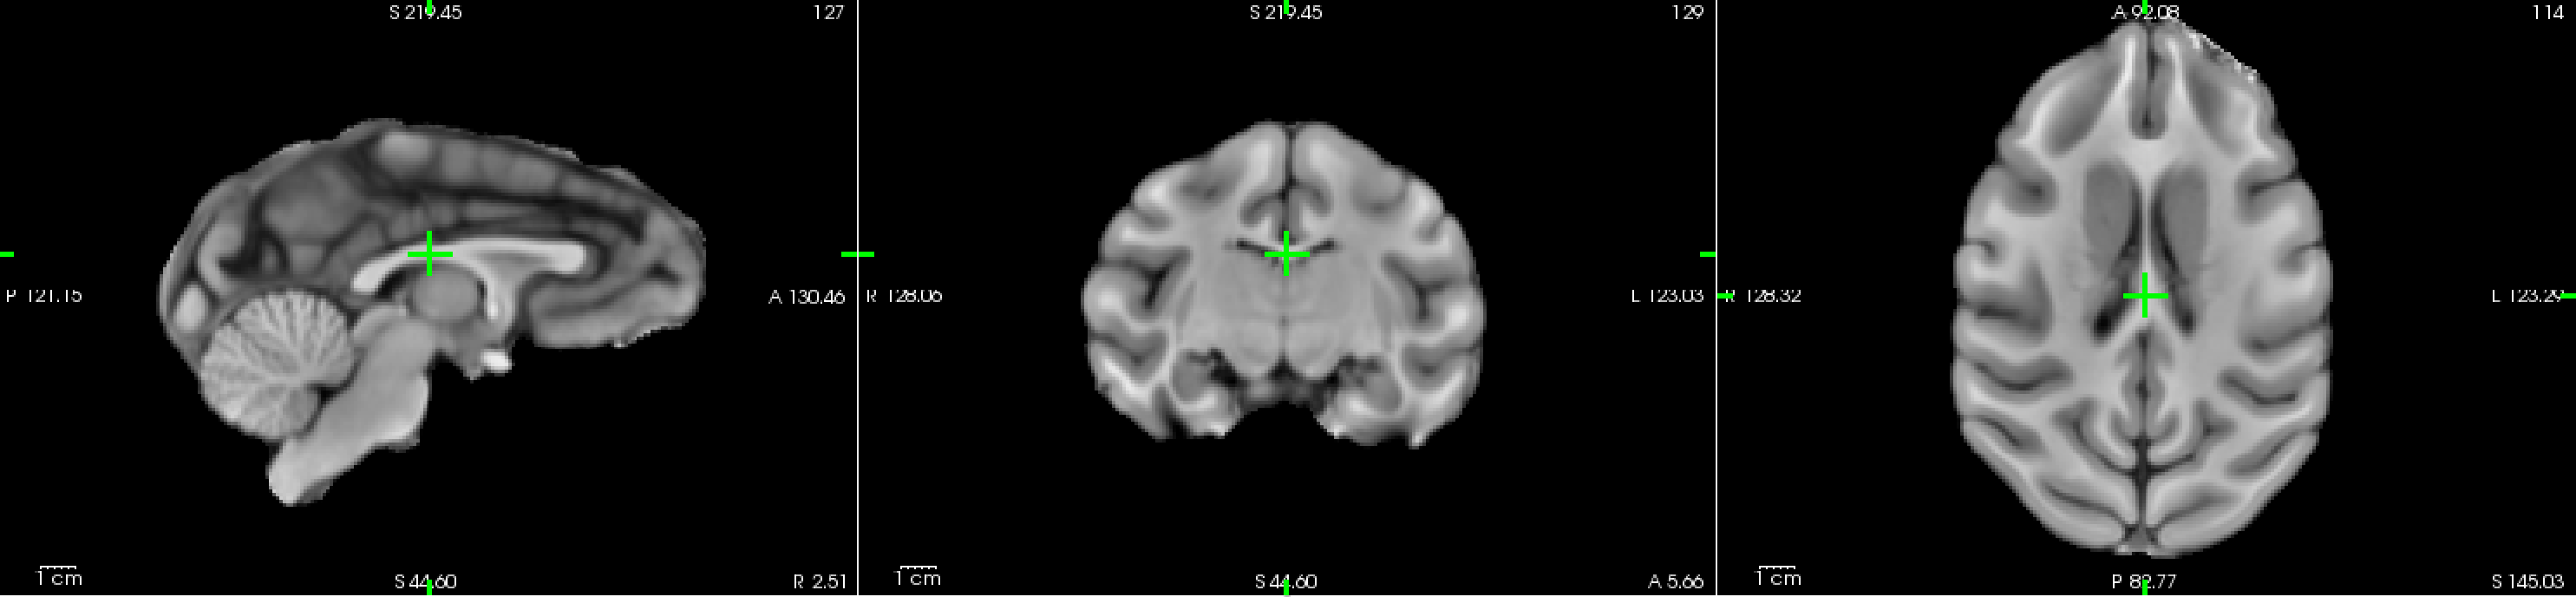
\includegraphics{pics/CC_coordinates.png}

Pons: 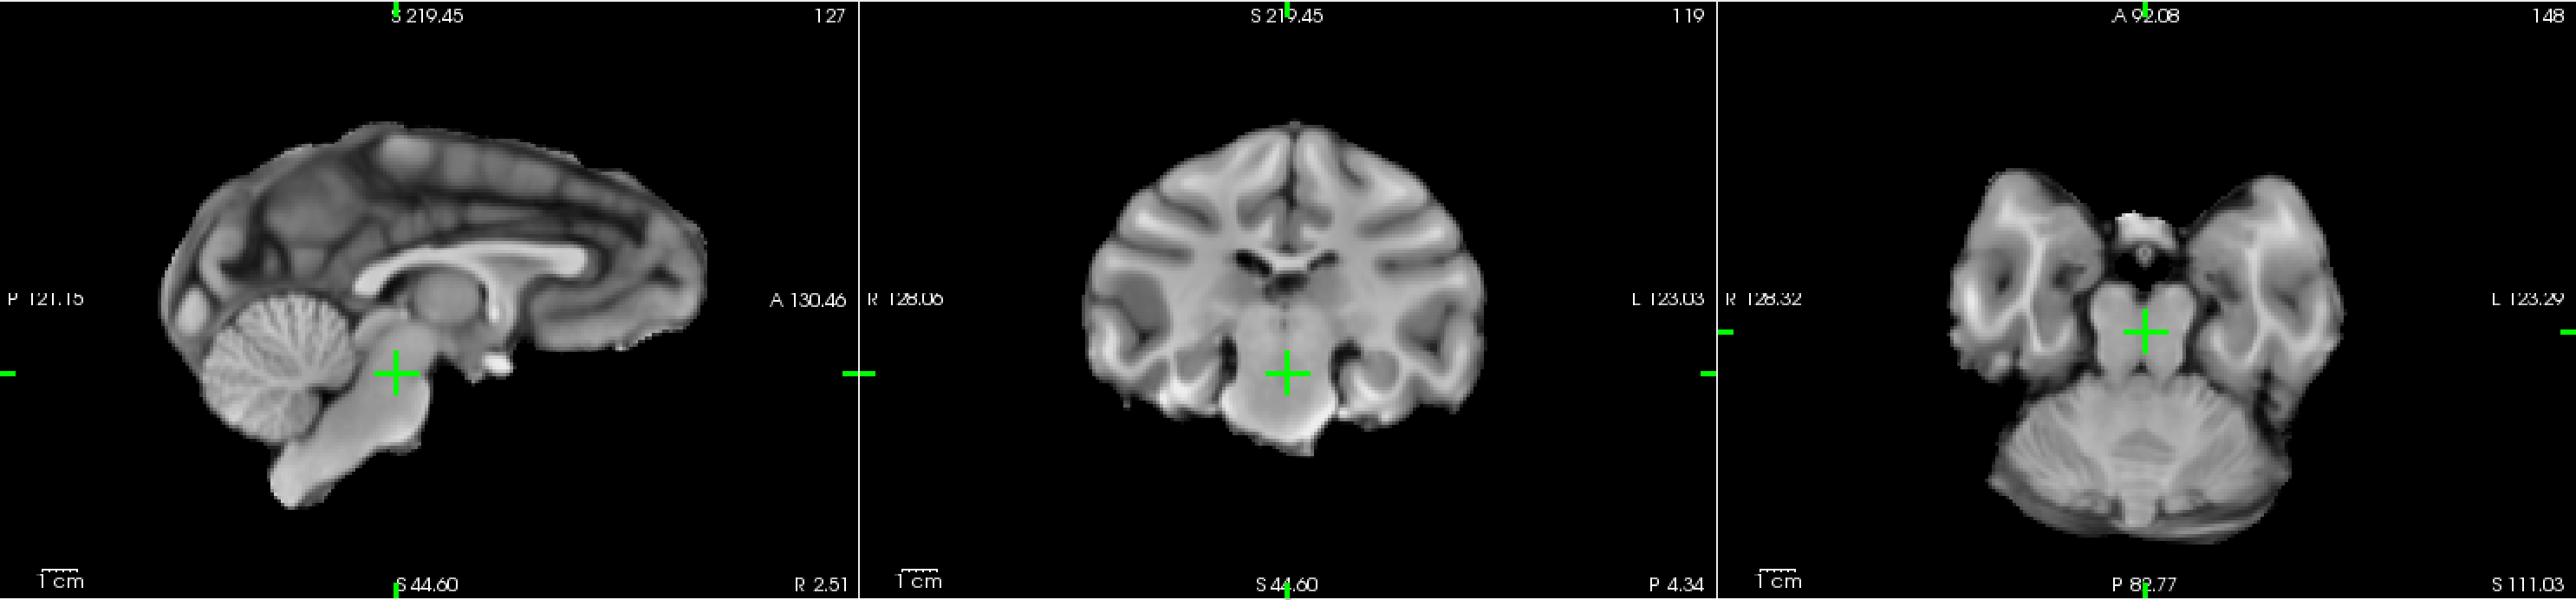
\includegraphics{pics/PONS_coordinates.png}

    \begin{Verbatim}[commandchars=\\\{\}]
{\color{incolor}In [{\color{incolor} }]:} \PY{c+c1}{\PYZsh{} Inspect volume to get voxel coordinates}
        freeview \PYZhy{}v \PY{l+s+si}{\PYZdl{}\PYZob{}}\PY{n+nv}{fsSurf\PYZus{}mgz}\PY{l+s+si}{\PYZcb{}}/brain.mgz \PY{p}{\PYZam{}}
\end{Verbatim}


    \begin{Verbatim}[commandchars=\\\{\}]
{\color{incolor}In [{\color{incolor} }]:} \PY{n+nv}{CC}\PY{o}{=}\PY{o}{(}\PY{l+m}{127} \PY{l+m}{114} \PY{l+m}{129}\PY{o}{)}
        \PY{n+nv}{PONS}\PY{o}{=}\PY{o}{(}\PY{l+m}{124} \PY{l+m}{148} \PY{l+m}{119}\PY{o}{)}
\end{Verbatim}


    \hypertarget{fill-the-white-matter-volume-copy-for-fixing}{%
\paragraph{Fill the white matter volume \& copy for
fixing}\label{fill-the-white-matter-volume-copy-for-fixing}}

    \begin{Verbatim}[commandchars=\\\{\}]
{\color{incolor}In [{\color{incolor} }]:} \PY{c+c1}{\PYZsh{} Fill WM}
        mri\PYZus{}fill \PYZhy{}CV \PY{l+s+si}{\PYZdl{}\PYZob{}}\PY{n+nv}{CC}\PY{p}{[0]}\PY{l+s+si}{\PYZcb{}} \PY{l+s+si}{\PYZdl{}\PYZob{}}\PY{n+nv}{CC}\PY{p}{[1]}\PY{l+s+si}{\PYZcb{}} \PY{l+s+si}{\PYZdl{}\PYZob{}}\PY{n+nv}{CC}\PY{p}{[2]}\PY{l+s+si}{\PYZcb{}} \PY{l+s+se}{\PYZbs{}}
            \PYZhy{}PV \PY{l+s+si}{\PYZdl{}\PYZob{}}\PY{n+nv}{PONS}\PY{p}{[0]}\PY{l+s+si}{\PYZcb{}} \PY{l+s+si}{\PYZdl{}\PYZob{}}\PY{n+nv}{PONS}\PY{p}{[1]}\PY{l+s+si}{\PYZcb{}} \PY{l+s+si}{\PYZdl{}\PYZob{}}\PY{n+nv}{PONS}\PY{p}{[2]}\PY{l+s+si}{\PYZcb{}} \PY{l+s+se}{\PYZbs{}}
            \PY{l+s+si}{\PYZdl{}\PYZob{}}\PY{n+nv}{fsSurf\PYZus{}mgz}\PY{l+s+si}{\PYZcb{}}/wm.mgz \PY{l+s+si}{\PYZdl{}\PYZob{}}\PY{n+nv}{fsSurf\PYZus{}mgz}\PY{l+s+si}{\PYZcb{}}/filled.mgz
            
        cp \PY{l+s+si}{\PYZdl{}\PYZob{}}\PY{n+nv}{fsSurf\PYZus{}mgz}\PY{l+s+si}{\PYZcb{}}/wm.mgz \PY{l+s+si}{\PYZdl{}\PYZob{}}\PY{n+nv}{fsSurf\PYZus{}mgz}\PY{l+s+si}{\PYZcb{}}/wm\PYZus{}nofix.mgz
\end{Verbatim}


    \hypertarget{tesselate-volumes-fix-topology-first-run}{%
\paragraph{Tesselate volumes \& fix topology (First
run)}\label{tesselate-volumes-fix-topology-first-run}}

    \begin{Verbatim}[commandchars=\\\{\}]
{\color{incolor}In [{\color{incolor} }]:} \PY{c+c1}{\PYZsh{} left}
        mri\PYZus{}pretess \PY{l+s+si}{\PYZdl{}\PYZob{}}\PY{n+nv}{fsSurf\PYZus{}mgz}\PY{l+s+si}{\PYZcb{}}/filled.mgz \PY{l+m}{255} \PY{l+s+si}{\PYZdl{}\PYZob{}}\PY{n+nv}{fsSurf\PYZus{}mgz}\PY{l+s+si}{\PYZcb{}}/brain.mgz \PY{l+s+si}{\PYZdl{}\PYZob{}}\PY{n+nv}{fsSurf\PYZus{}mgz}\PY{l+s+si}{\PYZcb{}}/wm\PYZus{}filled\PYZhy{}pretess255.mgz
        mri\PYZus{}tessellate \PY{l+s+si}{\PYZdl{}\PYZob{}}\PY{n+nv}{fsSurf\PYZus{}mgz}\PY{l+s+si}{\PYZcb{}}/wm\PYZus{}filled\PYZhy{}pretess255.mgz \PY{l+m}{255} \PY{l+s+si}{\PYZdl{}\PYZob{}}\PY{n+nv}{fsSurf\PYZus{}temp}\PY{l+s+si}{\PYZcb{}}/lh.orig.nofix
        \PY{c+c1}{\PYZsh{} right}
        mri\PYZus{}pretess \PY{l+s+si}{\PYZdl{}\PYZob{}}\PY{n+nv}{fsSurf\PYZus{}mgz}\PY{l+s+si}{\PYZcb{}}/filled.mgz \PY{l+m}{127} \PY{l+s+si}{\PYZdl{}\PYZob{}}\PY{n+nv}{fsSurf\PYZus{}mgz}\PY{l+s+si}{\PYZcb{}}/brain.mgz \PY{l+s+si}{\PYZdl{}\PYZob{}}\PY{n+nv}{fsSurf\PYZus{}mgz}\PY{l+s+si}{\PYZcb{}}/wm\PYZus{}filled\PYZhy{}pretess127.mgz
        mri\PYZus{}tessellate \PY{l+s+si}{\PYZdl{}\PYZob{}}\PY{n+nv}{fsSurf\PYZus{}mgz}\PY{l+s+si}{\PYZcb{}}/wm\PYZus{}filled\PYZhy{}pretess127.mgz \PY{l+m}{127} \PY{l+s+si}{\PYZdl{}\PYZob{}}\PY{n+nv}{fsSurf\PYZus{}temp}\PY{l+s+si}{\PYZcb{}}/rh.orig.nofix
        
        \PY{n+nv}{HEMI}\PY{o}{=}\PY{o}{(}lh rh\PY{o}{)} \PY{c+c1}{\PYZsh{} array to loop over hemispheres}
        \PY{k}{for} xh in \PY{l+s+si}{\PYZdl{}\PYZob{}}\PY{n+nv}{HEMI}\PY{p}{[@]}\PY{l+s+si}{\PYZcb{}}\PY{p}{;} \PY{k}{do}
            cp \PY{l+s+si}{\PYZdl{}\PYZob{}}\PY{n+nv}{fsSurf\PYZus{}temp}\PY{l+s+si}{\PYZcb{}}/\PY{l+s+si}{\PYZdl{}\PYZob{}}\PY{n+nv}{xh}\PY{l+s+si}{\PYZcb{}}.orig.nofix \PY{l+s+si}{\PYZdl{}\PYZob{}}\PY{n+nv}{fsSurf\PYZus{}temp}\PY{l+s+si}{\PYZcb{}}/\PY{l+s+si}{\PYZdl{}\PYZob{}}\PY{n+nv}{xh}\PY{l+s+si}{\PYZcb{}}.orig
        
            \PY{c+c1}{\PYZsh{} post\PYZhy{}process tesselation}
            mris\PYZus{}extract\PYZus{}main\PYZus{}component \PY{l+s+si}{\PYZdl{}\PYZob{}}\PY{n+nv}{fsSurf\PYZus{}temp}\PY{l+s+si}{\PYZcb{}}/\PY{l+s+si}{\PYZdl{}\PYZob{}}\PY{n+nv}{xh}\PY{l+s+si}{\PYZcb{}}.orig.nofix \PY{l+s+si}{\PYZdl{}\PYZob{}}\PY{n+nv}{fsSurf\PYZus{}temp}\PY{l+s+si}{\PYZcb{}}/\PY{l+s+si}{\PYZdl{}\PYZob{}}\PY{n+nv}{xh}\PY{l+s+si}{\PYZcb{}}.orig.nofix
            mris\PYZus{}smooth \PYZhy{}nw \PY{l+s+si}{\PYZdl{}\PYZob{}}\PY{n+nv}{fsSurf\PYZus{}temp}\PY{l+s+si}{\PYZcb{}}/\PY{l+s+si}{\PYZdl{}\PYZob{}}\PY{n+nv}{xh}\PY{l+s+si}{\PYZcb{}}.orig.nofix \PY{l+s+si}{\PYZdl{}\PYZob{}}\PY{n+nv}{fsSurf\PYZus{}temp}\PY{l+s+si}{\PYZcb{}}/\PY{l+s+si}{\PYZdl{}\PYZob{}}\PY{n+nv}{xh}\PY{l+s+si}{\PYZcb{}}.smoothwm.nofix
            mris\PYZus{}inflate \PY{l+s+si}{\PYZdl{}\PYZob{}}\PY{n+nv}{fsSurf\PYZus{}temp}\PY{l+s+si}{\PYZcb{}}/\PY{l+s+si}{\PYZdl{}\PYZob{}}\PY{n+nv}{xh}\PY{l+s+si}{\PYZcb{}}.smoothwm.nofix \PY{l+s+si}{\PYZdl{}\PYZob{}}\PY{n+nv}{fsSurf\PYZus{}temp}\PY{l+s+si}{\PYZcb{}}/\PY{l+s+si}{\PYZdl{}\PYZob{}}\PY{n+nv}{xh}\PY{l+s+si}{\PYZcb{}}.inflated.nofix
            mris\PYZus{}sphere \PYZhy{}q \PY{l+s+si}{\PYZdl{}\PYZob{}}\PY{n+nv}{fsSurf\PYZus{}temp}\PY{l+s+si}{\PYZcb{}}/\PY{l+s+si}{\PYZdl{}\PYZob{}}\PY{n+nv}{xh}\PY{l+s+si}{\PYZcb{}}.inflated.nofix \PY{l+s+si}{\PYZdl{}\PYZob{}}\PY{n+nv}{fsSurf\PYZus{}temp}\PY{l+s+si}{\PYZcb{}}/\PY{l+s+si}{\PYZdl{}\PYZob{}}\PY{n+nv}{xh}\PY{l+s+si}{\PYZcb{}}.qsphere.nofix
            cp \PY{l+s+si}{\PYZdl{}\PYZob{}}\PY{n+nv}{fsSurf\PYZus{}temp}\PY{l+s+si}{\PYZcb{}}/\PY{l+s+si}{\PYZdl{}\PYZob{}}\PY{n+nv}{xh}\PY{l+s+si}{\PYZcb{}}.inflated.nofix \PY{l+s+si}{\PYZdl{}\PYZob{}}\PY{n+nv}{fsSurf\PYZus{}temp}\PY{l+s+si}{\PYZcb{}}/\PY{l+s+si}{\PYZdl{}\PYZob{}}\PY{n+nv}{xh}\PY{l+s+si}{\PYZcb{}}.inflated
        
            \PY{c+c1}{\PYZsh{} fix topology}
            mris\PYZus{}euler\PYZus{}number \PY{l+s+si}{\PYZdl{}\PYZob{}}\PY{n+nv}{fsSurf\PYZus{}temp}\PY{l+s+si}{\PYZcb{}}/\PY{l+s+si}{\PYZdl{}\PYZob{}}\PY{n+nv}{xh}\PY{l+s+si}{\PYZcb{}}.orig
            mris\PYZus{}remove\PYZus{}intersection \PY{l+s+si}{\PYZdl{}\PYZob{}}\PY{n+nv}{fsSurf\PYZus{}temp}\PY{l+s+si}{\PYZcb{}}/\PY{l+s+si}{\PYZdl{}\PYZob{}}\PY{n+nv}{xh}\PY{l+s+si}{\PYZcb{}}.orig \PY{l+s+si}{\PYZdl{}\PYZob{}}\PY{n+nv}{fsSurf\PYZus{}temp}\PY{l+s+si}{\PYZcb{}}/\PY{l+s+si}{\PYZdl{}\PYZob{}}\PY{n+nv}{xh}\PY{l+s+si}{\PYZcb{}}.orig
            mris\PYZus{}smooth \PYZhy{}nw \PY{l+s+si}{\PYZdl{}\PYZob{}}\PY{n+nv}{fsSurf\PYZus{}temp}\PY{l+s+si}{\PYZcb{}}/\PY{l+s+si}{\PYZdl{}\PYZob{}}\PY{n+nv}{xh}\PY{l+s+si}{\PYZcb{}}.orig \PY{l+s+si}{\PYZdl{}\PYZob{}}\PY{n+nv}{fsSurf\PYZus{}temp}\PY{l+s+si}{\PYZcb{}}/\PY{l+s+si}{\PYZdl{}\PYZob{}}\PY{n+nv}{xh}\PY{l+s+si}{\PYZcb{}}.smoothwm
            mris\PYZus{}inflate \PY{l+s+si}{\PYZdl{}\PYZob{}}\PY{n+nv}{fsSurf\PYZus{}temp}\PY{l+s+si}{\PYZcb{}}/\PY{l+s+si}{\PYZdl{}\PYZob{}}\PY{n+nv}{xh}\PY{l+s+si}{\PYZcb{}}.smoothwm \PY{l+s+si}{\PYZdl{}\PYZob{}}\PY{n+nv}{fsSurf\PYZus{}temp}\PY{l+s+si}{\PYZcb{}}/\PY{l+s+si}{\PYZdl{}\PYZob{}}\PY{n+nv}{xh}\PY{l+s+si}{\PYZcb{}}.inflated
        \PY{k}{done}
\end{Verbatim}


    \hypertarget{iterate-manual-adjustments-and-doing-tesselation-topology-fix-again}{%
\paragraph{Iterate manual adjustments and doing tesselation \& topology
fix
again}\label{iterate-manual-adjustments-and-doing-tesselation-topology-fix-again}}

Should look something like this. Keep going (adjust wm.mgz using the
recon-edit function of Freeview) until you are happy with the result.

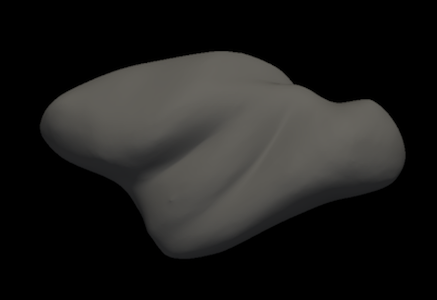
\includegraphics{pics/LH_wm_inflated.png}
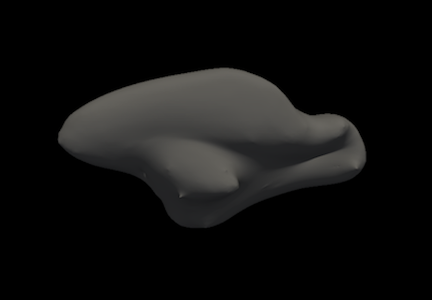
\includegraphics{pics/RH_in_wm_inflated.png}

    \begin{Verbatim}[commandchars=\\\{\}]
{\color{incolor}In [{\color{incolor} }]:} \PY{c+c1}{\PYZsh{} look at the result and apply fixes in WM definition}
        freeview \PYZhy{}v \PY{l+s+si}{\PYZdl{}\PYZob{}}\PY{n+nv}{fsSurf\PYZus{}mgz}\PY{l+s+si}{\PYZcb{}}/brain.mgz \PYZhy{}v \PY{l+s+si}{\PYZdl{}\PYZob{}}\PY{n+nv}{fsSurf\PYZus{}mgz}\PY{l+s+si}{\PYZcb{}}/wm.mgz \PY{l+s+se}{\PYZbs{}}
            \PYZhy{}f \PY{l+s+si}{\PYZdl{}\PYZob{}}\PY{n+nv}{fsSurf\PYZus{}temp}\PY{l+s+si}{\PYZcb{}}/lh.smoothwm \PY{l+s+si}{\PYZdl{}\PYZob{}}\PY{n+nv}{fsSurf\PYZus{}temp}\PY{l+s+si}{\PYZcb{}}/lh.inflated \PY{l+s+se}{\PYZbs{}}
            \PY{l+s+si}{\PYZdl{}\PYZob{}}\PY{n+nv}{fsSurf\PYZus{}temp}\PY{l+s+si}{\PYZcb{}}/rh.smoothwm \PY{l+s+si}{\PYZdl{}\PYZob{}}\PY{n+nv}{fsSurf\PYZus{}temp}\PY{l+s+si}{\PYZcb{}}/rh.inflated \PY{p}{\PYZam{}}
\end{Verbatim}


    \begin{Verbatim}[commandchars=\\\{\}]
{\color{incolor}In [{\color{incolor} }]:} \PY{c+c1}{\PYZsh{} redo the tesselation with the fixed WM volume}
        mri\PYZus{}fill \PYZhy{}CV \PY{l+s+si}{\PYZdl{}\PYZob{}}\PY{n+nv}{CC}\PY{p}{[0]}\PY{l+s+si}{\PYZcb{}} \PY{l+s+si}{\PYZdl{}\PYZob{}}\PY{n+nv}{CC}\PY{p}{[1]}\PY{l+s+si}{\PYZcb{}} \PY{l+s+si}{\PYZdl{}\PYZob{}}\PY{n+nv}{CC}\PY{p}{[2]}\PY{l+s+si}{\PYZcb{}} \PY{l+s+se}{\PYZbs{}}
            \PYZhy{}PV \PY{l+s+si}{\PYZdl{}\PYZob{}}\PY{n+nv}{PONS}\PY{p}{[0]}\PY{l+s+si}{\PYZcb{}} \PY{l+s+si}{\PYZdl{}\PYZob{}}\PY{n+nv}{PONS}\PY{p}{[1]}\PY{l+s+si}{\PYZcb{}} \PY{l+s+si}{\PYZdl{}\PYZob{}}\PY{n+nv}{PONS}\PY{p}{[2]}\PY{l+s+si}{\PYZcb{}} \PY{l+s+se}{\PYZbs{}}
            \PY{l+s+si}{\PYZdl{}\PYZob{}}\PY{n+nv}{fsSurf\PYZus{}mgz}\PY{l+s+si}{\PYZcb{}}/wm.mgz \PY{l+s+si}{\PYZdl{}\PYZob{}}\PY{n+nv}{fsSurf\PYZus{}mgz}\PY{l+s+si}{\PYZcb{}}/filled.mgz
            
        mri\PYZus{}pretess \PY{l+s+si}{\PYZdl{}\PYZob{}}\PY{n+nv}{fsSurf\PYZus{}mgz}\PY{l+s+si}{\PYZcb{}}/filled.mgz \PY{l+m}{255} \PY{l+s+si}{\PYZdl{}\PYZob{}}\PY{n+nv}{fsSurf\PYZus{}mgz}\PY{l+s+si}{\PYZcb{}}/brain.mgz \PY{l+s+si}{\PYZdl{}\PYZob{}}\PY{n+nv}{fsSurf\PYZus{}mgz}\PY{l+s+si}{\PYZcb{}}/wm\PYZus{}filled\PYZhy{}pretess255.mgz
        mri\PYZus{}tessellate \PY{l+s+si}{\PYZdl{}\PYZob{}}\PY{n+nv}{fsSurf\PYZus{}mgz}\PY{l+s+si}{\PYZcb{}}/wm\PYZus{}filled\PYZhy{}pretess255.mgz \PY{l+m}{255} \PY{l+s+si}{\PYZdl{}\PYZob{}}\PY{n+nv}{fsSurf\PYZus{}temp}\PY{l+s+si}{\PYZcb{}}/lh.orig
        mri\PYZus{}pretess \PY{l+s+si}{\PYZdl{}\PYZob{}}\PY{n+nv}{fsSurf\PYZus{}mgz}\PY{l+s+si}{\PYZcb{}}/filled.mgz \PY{l+m}{127} \PY{l+s+si}{\PYZdl{}\PYZob{}}\PY{n+nv}{fsSurf\PYZus{}mgz}\PY{l+s+si}{\PYZcb{}}/brain.mgz \PY{l+s+si}{\PYZdl{}\PYZob{}}\PY{n+nv}{fsSurf\PYZus{}mgz}\PY{l+s+si}{\PYZcb{}}/wm\PYZus{}filled\PYZhy{}pretess127.mgz
        mri\PYZus{}tessellate \PY{l+s+si}{\PYZdl{}\PYZob{}}\PY{n+nv}{fsSurf\PYZus{}mgz}\PY{l+s+si}{\PYZcb{}}/wm\PYZus{}filled\PYZhy{}pretess127.mgz \PY{l+m}{127} \PY{l+s+si}{\PYZdl{}\PYZob{}}\PY{n+nv}{fsSurf\PYZus{}temp}\PY{l+s+si}{\PYZcb{}}/rh.orig
        
        \PY{k}{for} xh in \PY{l+s+si}{\PYZdl{}\PYZob{}}\PY{n+nv}{HEMI}\PY{p}{[@]}\PY{l+s+si}{\PYZcb{}}\PY{p}{;} \PY{k}{do}
            mris\PYZus{}extract\PYZus{}main\PYZus{}component \PY{l+s+si}{\PYZdl{}\PYZob{}}\PY{n+nv}{fsSurf\PYZus{}temp}\PY{l+s+si}{\PYZcb{}}/\PY{l+s+si}{\PYZdl{}\PYZob{}}\PY{n+nv}{xh}\PY{l+s+si}{\PYZcb{}}.orig \PY{l+s+si}{\PYZdl{}\PYZob{}}\PY{n+nv}{fsSurf\PYZus{}temp}\PY{l+s+si}{\PYZcb{}}/\PY{l+s+si}{\PYZdl{}\PYZob{}}\PY{n+nv}{xh}\PY{l+s+si}{\PYZcb{}}.orig
            mris\PYZus{}smooth \PYZhy{}nw \PY{l+s+si}{\PYZdl{}\PYZob{}}\PY{n+nv}{fsSurf\PYZus{}temp}\PY{l+s+si}{\PYZcb{}}/\PY{l+s+si}{\PYZdl{}\PYZob{}}\PY{n+nv}{xh}\PY{l+s+si}{\PYZcb{}}.orig \PY{l+s+si}{\PYZdl{}\PYZob{}}\PY{n+nv}{fsSurf\PYZus{}temp}\PY{l+s+si}{\PYZcb{}}/\PY{l+s+si}{\PYZdl{}\PYZob{}}\PY{n+nv}{xh}\PY{l+s+si}{\PYZcb{}}.smoothwm
            mris\PYZus{}inflate \PY{l+s+si}{\PYZdl{}\PYZob{}}\PY{n+nv}{fsSurf\PYZus{}temp}\PY{l+s+si}{\PYZcb{}}/\PY{l+s+si}{\PYZdl{}\PYZob{}}\PY{n+nv}{xh}\PY{l+s+si}{\PYZcb{}}.smoothwm \PY{l+s+si}{\PYZdl{}\PYZob{}}\PY{n+nv}{fsSurf\PYZus{}temp}\PY{l+s+si}{\PYZcb{}}/\PY{l+s+si}{\PYZdl{}\PYZob{}}\PY{n+nv}{xh}\PY{l+s+si}{\PYZcb{}}.inflated
            mris\PYZus{}sphere \PYZhy{}q \PY{l+s+si}{\PYZdl{}\PYZob{}}\PY{n+nv}{fsSurf\PYZus{}temp}\PY{l+s+si}{\PYZcb{}}/\PY{l+s+si}{\PYZdl{}\PYZob{}}\PY{n+nv}{xh}\PY{l+s+si}{\PYZcb{}}.inflated \PY{l+s+si}{\PYZdl{}\PYZob{}}\PY{n+nv}{fsSurf\PYZus{}temp}\PY{l+s+si}{\PYZcb{}}/\PY{l+s+si}{\PYZdl{}\PYZob{}}\PY{n+nv}{xh}\PY{l+s+si}{\PYZcb{}}.qsphere
            
            mris\PYZus{}euler\PYZus{}number \PY{l+s+si}{\PYZdl{}\PYZob{}}\PY{n+nv}{fsSurf\PYZus{}temp}\PY{l+s+si}{\PYZcb{}}/\PY{l+s+si}{\PYZdl{}\PYZob{}}\PY{n+nv}{xh}\PY{l+s+si}{\PYZcb{}}.orig
            mris\PYZus{}remove\PYZus{}intersection \PY{l+s+si}{\PYZdl{}\PYZob{}}\PY{n+nv}{fsSurf\PYZus{}temp}\PY{l+s+si}{\PYZcb{}}/\PY{l+s+si}{\PYZdl{}\PYZob{}}\PY{n+nv}{xh}\PY{l+s+si}{\PYZcb{}}.orig \PY{l+s+si}{\PYZdl{}\PYZob{}}\PY{n+nv}{fsSurf\PYZus{}temp}\PY{l+s+si}{\PYZcb{}}/\PY{l+s+si}{\PYZdl{}\PYZob{}}\PY{n+nv}{xh}\PY{l+s+si}{\PYZcb{}}.orig
            mris\PYZus{}smooth \PYZhy{}nw \PY{l+s+si}{\PYZdl{}\PYZob{}}\PY{n+nv}{fsSurf\PYZus{}temp}\PY{l+s+si}{\PYZcb{}}/\PY{l+s+si}{\PYZdl{}\PYZob{}}\PY{n+nv}{xh}\PY{l+s+si}{\PYZcb{}}.orig \PY{l+s+si}{\PYZdl{}\PYZob{}}\PY{n+nv}{fsSurf\PYZus{}temp}\PY{l+s+si}{\PYZcb{}}/\PY{l+s+si}{\PYZdl{}\PYZob{}}\PY{n+nv}{xh}\PY{l+s+si}{\PYZcb{}}.smoothwm
            mris\PYZus{}inflate \PY{l+s+si}{\PYZdl{}\PYZob{}}\PY{n+nv}{fsSurf\PYZus{}temp}\PY{l+s+si}{\PYZcb{}}/\PY{l+s+si}{\PYZdl{}\PYZob{}}\PY{n+nv}{xh}\PY{l+s+si}{\PYZcb{}}.smoothwm \PY{l+s+si}{\PYZdl{}\PYZob{}}\PY{n+nv}{fsSurf\PYZus{}temp}\PY{l+s+si}{\PYZcb{}}/\PY{l+s+si}{\PYZdl{}\PYZob{}}\PY{n+nv}{xh}\PY{l+s+si}{\PYZcb{}}.inflated
            mris\PYZus{}curvature \PYZhy{}thresh .999 \PYZhy{}n \PYZhy{}a \PY{l+m}{5} \PYZhy{}w \PYZhy{}distances \PY{l+m}{10} \PY{l+m}{10} \PY{l+s+si}{\PYZdl{}\PYZob{}}\PY{n+nv}{fsSurf\PYZus{}temp}\PY{l+s+si}{\PYZcb{}}/\PY{l+s+si}{\PYZdl{}\PYZob{}}\PY{n+nv}{xh}\PY{l+s+si}{\PYZcb{}}.inflated
            mris\PYZus{}sphere \PY{l+s+si}{\PYZdl{}\PYZob{}}\PY{n+nv}{fsSurf\PYZus{}temp}\PY{l+s+si}{\PYZcb{}}/\PY{l+s+si}{\PYZdl{}\PYZob{}}\PY{n+nv}{xh}\PY{l+s+si}{\PYZcb{}}.inflated \PY{l+s+si}{\PYZdl{}\PYZob{}}\PY{n+nv}{fsSurf\PYZus{}temp}\PY{l+s+si}{\PYZcb{}}/\PY{l+s+si}{\PYZdl{}\PYZob{}}\PY{n+nv}{xh}\PY{l+s+si}{\PYZcb{}}.sphere
        \PY{k}{done}
        \PY{n+nb}{echo} \PY{l+s+s1}{\PYZsq{}TESSELATION DONE!\PYZsq{}}
\end{Verbatim}


    \begin{Verbatim}[commandchars=\\\{\}]
{\color{incolor}In [{\color{incolor} }]:} \PY{k}{for} xh in \PY{l+s+si}{\PYZdl{}\PYZob{}}\PY{n+nv}{HEMI}\PY{p}{[@]}\PY{l+s+si}{\PYZcb{}}\PY{p}{;} \PY{k}{do}
            mris\PYZus{}sphere \PY{l+s+si}{\PYZdl{}\PYZob{}}\PY{n+nv}{fsSurf\PYZus{}temp}\PY{l+s+si}{\PYZcb{}}/\PY{l+s+si}{\PYZdl{}\PYZob{}}\PY{n+nv}{xh}\PY{l+s+si}{\PYZcb{}}.inflated \PY{l+s+si}{\PYZdl{}\PYZob{}}\PY{n+nv}{fsSurf\PYZus{}temp}\PY{l+s+si}{\PYZcb{}}/\PY{l+s+si}{\PYZdl{}\PYZob{}}\PY{n+nv}{xh}\PY{l+s+si}{\PYZcb{}}.sphere
        \PY{k}{done}
\end{Verbatim}


    \hypertarget{create-a-subject-directory-in-your-freesurfer-subject-directory}{%
\paragraph{Create a subject directory in your freesurfer subject
directory}\label{create-a-subject-directory-in-your-freesurfer-subject-directory}}

    \begin{Verbatim}[commandchars=\\\{\}]
{\color{incolor}In [{\color{incolor} }]:} \PY{c+c1}{\PYZsh{} create a freesurfer SUBJECT with the correct folder structure}
        \PY{c+c1}{\PYZsh{} NB! \PYZdl{}SUBJECTS\PYZus{}DIR should be defined in your \PYZti{}/.bashrc as the Freesurfer subjects directory}
        \PY{n+nb}{echo} \PY{l+s+s1}{\PYZsq{}Creating a subject directory for \PYZsq{}}\PY{l+s+si}{\PYZdl{}\PYZob{}}\PY{n+nv}{SUBJ}\PY{l+s+si}{\PYZcb{}}\PY{l+s+s1}{\PYZsq{}in:\PYZsq{}}
        \PY{n+nb}{echo} \PY{l+s+si}{\PYZdl{}\PYZob{}}\PY{n+nv}{SUBJECTS\PYZus{}DIR}\PY{l+s+si}{\PYZcb{}}/\PY{l+s+si}{\PYZdl{}\PYZob{}}\PY{n+nv}{SUBJ}\PY{l+s+si}{\PYZcb{}}
        mksubjdirs \PY{l+s+si}{\PYZdl{}\PYZob{}}\PY{n+nv}{SUBJECTS\PYZus{}DIR}\PY{l+s+si}{\PYZcb{}}/\PY{l+s+si}{\PYZdl{}\PYZob{}}\PY{n+nv}{SUBJ}\PY{l+s+si}{\PYZcb{}}
\end{Verbatim}


    \hypertarget{cut-surfaces-and-create-flatmaps}{%
\paragraph{Cut surfaces and create
flatmaps}\label{cut-surfaces-and-create-flatmaps}}

    \begin{Verbatim}[commandchars=\\\{\}]
{\color{incolor}In [{\color{incolor} }]:} \PY{c+c1}{\PYZsh{} copy the necessary files for cutting to the subject directory}
        \PY{k}{for} xh in \PY{l+s+si}{\PYZdl{}\PYZob{}}\PY{n+nv}{HEMI}\PY{p}{[@]}\PY{l+s+si}{\PYZcb{}}\PY{p}{;} \PY{k}{do}
            cp \PY{l+s+si}{\PYZdl{}\PYZob{}}\PY{n+nv}{fsSurf\PYZus{}temp}\PY{l+s+si}{\PYZcb{}}/\PY{l+s+si}{\PYZdl{}\PYZob{}}\PY{n+nv}{xh}\PY{l+s+si}{\PYZcb{}}.inflated \PY{l+s+si}{\PYZdl{}\PYZob{}}\PY{n+nv}{SUBJECTS\PYZus{}DIR}\PY{l+s+si}{\PYZcb{}}/\PY{l+s+si}{\PYZdl{}\PYZob{}}\PY{n+nv}{SUBJ}\PY{l+s+si}{\PYZcb{}}/surf/
            cp \PY{l+s+si}{\PYZdl{}\PYZob{}}\PY{n+nv}{fsSurf\PYZus{}temp}\PY{l+s+si}{\PYZcb{}}/\PY{l+s+si}{\PYZdl{}\PYZob{}}\PY{n+nv}{xh}\PY{l+s+si}{\PYZcb{}}.smoothwm \PY{l+s+si}{\PYZdl{}\PYZob{}}\PY{n+nv}{SUBJECTS\PYZus{}DIR}\PY{l+s+si}{\PYZcb{}}/\PY{l+s+si}{\PYZdl{}\PYZob{}}\PY{n+nv}{SUBJ}\PY{l+s+si}{\PYZcb{}}/surf/
            cp \PY{l+s+si}{\PYZdl{}\PYZob{}}\PY{n+nv}{fsSurf\PYZus{}temp}\PY{l+s+si}{\PYZcb{}}/\PY{l+s+si}{\PYZdl{}\PYZob{}}\PY{n+nv}{xh}\PY{l+s+si}{\PYZcb{}}.orig \PY{l+s+si}{\PYZdl{}\PYZob{}}\PY{n+nv}{SUBJECTS\PYZus{}DIR}\PY{l+s+si}{\PYZcb{}}/\PY{l+s+si}{\PYZdl{}\PYZob{}}\PY{n+nv}{SUBJ}\PY{l+s+si}{\PYZcb{}}/surf/
            cp \PY{l+s+si}{\PYZdl{}\PYZob{}}\PY{n+nv}{fsSurf\PYZus{}temp}\PY{l+s+si}{\PYZcb{}}/\PY{l+s+si}{\PYZdl{}\PYZob{}}\PY{n+nv}{xh}\PY{l+s+si}{\PYZcb{}}.qsphere \PY{l+s+si}{\PYZdl{}\PYZob{}}\PY{n+nv}{SUBJECTS\PYZus{}DIR}\PY{l+s+si}{\PYZcb{}}/\PY{l+s+si}{\PYZdl{}\PYZob{}}\PY{n+nv}{SUBJ}\PY{l+s+si}{\PYZcb{}}/surf/
        \PY{k}{done}
        
        cp \PY{l+s+si}{\PYZdl{}\PYZob{}}\PY{n+nv}{fsSurf\PYZus{}mgz}\PY{l+s+si}{\PYZcb{}}/T1.mgz \PY{l+s+si}{\PYZdl{}\PYZob{}}\PY{n+nv}{SUBJECTS\PYZus{}DIR}\PY{l+s+si}{\PYZcb{}}/\PY{l+s+si}{\PYZdl{}\PYZob{}}\PY{n+nv}{SUBJ}\PY{l+s+si}{\PYZcb{}}/mri/T1.mgz
        cp \PY{l+s+si}{\PYZdl{}\PYZob{}}\PY{n+nv}{fsSurf\PYZus{}mgz}\PY{l+s+si}{\PYZcb{}}/filled.mgz \PY{l+s+si}{\PYZdl{}\PYZob{}}\PY{n+nv}{SUBJECTS\PYZus{}DIR}\PY{l+s+si}{\PYZcb{}}/\PY{l+s+si}{\PYZdl{}\PYZob{}}\PY{n+nv}{SUBJ}\PY{l+s+si}{\PYZcb{}}/mri/filled.mgz
        cp \PY{l+s+si}{\PYZdl{}\PYZob{}}\PY{n+nv}{fsSurf\PYZus{}mgz}\PY{l+s+si}{\PYZcb{}}/wm.mgz \PY{l+s+si}{\PYZdl{}\PYZob{}}\PY{n+nv}{SUBJECTS\PYZus{}DIR}\PY{l+s+si}{\PYZcb{}}/\PY{l+s+si}{\PYZdl{}\PYZob{}}\PY{n+nv}{SUBJ}\PY{l+s+si}{\PYZcb{}}/mri/wm.mgz
        cp \PY{l+s+si}{\PYZdl{}\PYZob{}}\PY{n+nv}{fsSurf\PYZus{}mgz}\PY{l+s+si}{\PYZcb{}}/brain.finalsurfs.mgz \PY{l+s+si}{\PYZdl{}\PYZob{}}\PY{n+nv}{SUBJECTS\PYZus{}DIR}\PY{l+s+si}{\PYZcb{}}/\PY{l+s+si}{\PYZdl{}\PYZob{}}\PY{n+nv}{SUBJ}\PY{l+s+si}{\PYZcb{}}/mri/brain.finalsurfs.mgz
\end{Verbatim}


    \begin{Verbatim}[commandchars=\\\{\}]
{\color{incolor}In [{\color{incolor} }]:} \PY{c+c1}{\PYZsh{} create surfaces}
        \PY{k}{for} xh in \PY{l+s+si}{\PYZdl{}\PYZob{}}\PY{n+nv}{HEMI}\PY{p}{[@]}\PY{l+s+si}{\PYZcb{}}\PY{p}{;} \PY{k}{do}
            mris\PYZus{}make\PYZus{}surfaces \PYZhy{}noaseg \PYZhy{}noaparc \PYZhy{}T1 brain.finalsurfs \PYZhy{}orig\PYZus{}wm orig \PY{l+s+si}{\PYZdl{}\PYZob{}}\PY{n+nv}{SUBJ}\PY{l+s+si}{\PYZcb{}} \PY{l+s+si}{\PYZdl{}\PYZob{}}\PY{n+nv}{xh}\PY{l+s+si}{\PYZcb{}}
            mris\PYZus{}sphere \PY{l+s+si}{\PYZdl{}\PYZob{}}\PY{n+nv}{SUBJECTS\PYZus{}DIR}\PY{l+s+si}{\PYZcb{}}/\PY{l+s+si}{\PYZdl{}\PYZob{}}\PY{n+nv}{SUBJ}\PY{l+s+si}{\PYZcb{}}/surf/\PY{l+s+si}{\PYZdl{}\PYZob{}}\PY{n+nv}{xh}\PY{l+s+si}{\PYZcb{}}.inflated \PY{l+s+si}{\PYZdl{}\PYZob{}}\PY{n+nv}{SUBJECTS\PYZus{}DIR}\PY{l+s+si}{\PYZcb{}}/\PY{l+s+si}{\PYZdl{}\PYZob{}}\PY{n+nv}{SUBJ}\PY{l+s+si}{\PYZcb{}}/surf/\PY{l+s+si}{\PYZdl{}\PYZob{}}\PY{n+nv}{xh}\PY{l+s+si}{\PYZcb{}}.sphere
            mris\PYZus{}expand \PYZhy{}thickness \PY{l+s+si}{\PYZdl{}\PYZob{}}\PY{n+nv}{SUBJECTS\PYZus{}DIR}\PY{l+s+si}{\PYZcb{}}/\PY{l+s+si}{\PYZdl{}\PYZob{}}\PY{n+nv}{SUBJ}\PY{l+s+si}{\PYZcb{}}/surf/\PY{l+s+si}{\PYZdl{}\PYZob{}}\PY{n+nv}{xh}\PY{l+s+si}{\PYZcb{}}.white \PY{l+m}{0}.5 \PY{l+s+si}{\PYZdl{}\PYZob{}}\PY{n+nv}{SUBJECTS\PYZus{}DIR}\PY{l+s+si}{\PYZcb{}}/\PY{l+s+si}{\PYZdl{}\PYZob{}}\PY{n+nv}{SUBJ}\PY{l+s+si}{\PYZcb{}}/surf/\PY{l+s+si}{\PYZdl{}\PYZob{}}\PY{n+nv}{xh}\PY{l+s+si}{\PYZcb{}}.graymid
        \PY{k}{done}
\end{Verbatim}


    The cells below will load the inflated hemispheres in tksurfer where you
can make the cuts to create the flatmaps.

For the full hemisphere make cuts on the medial wall. One cut enclosing
the midline and five additional relaxation cuts. Mark a point on the
part of the surface you want to keep and save patch as
\texttt{?h.full.patch.3d} (replace `?' with `l' and `r' respectively)

\begin{figure}
\centering
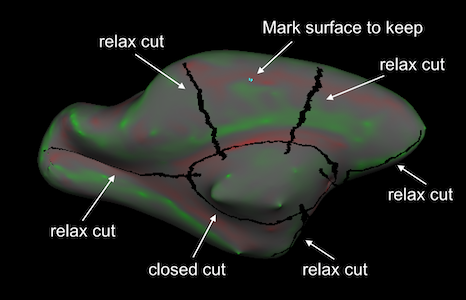
\includegraphics{pics/Cut_full.png}
\caption{Cut\_full}
\end{figure}

For an occipital patch make one cut on the medial wall along the
calcarine sulcus. Use 3 points to select a coronal cutting plane, and a
fourth point to select which part of the surface you want to keep and
save as \texttt{?h.occip.patch.3d}

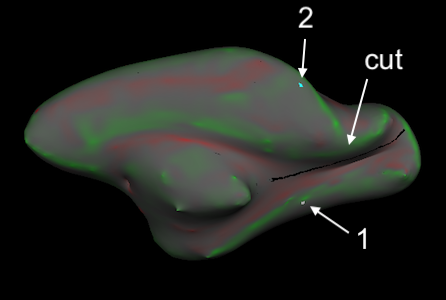
\includegraphics{pics/Cut_occip1.png}
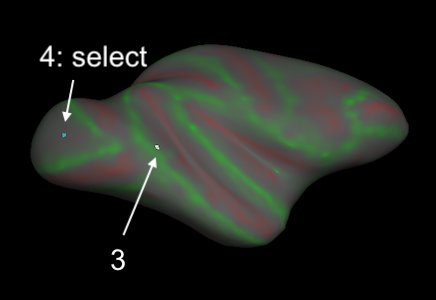
\includegraphics{pics/Cut_occip2.png}

    \begin{Verbatim}[commandchars=\\\{\}]
{\color{incolor}In [{\color{incolor} }]:} \PY{c+c1}{\PYZsh{} left}
        tksurfer \PY{l+s+si}{\PYZdl{}\PYZob{}}\PY{n+nv}{SUBJ}\PY{l+s+si}{\PYZcb{}} lh inflated \PYZhy{}curv
\end{Verbatim}


    \begin{Verbatim}[commandchars=\\\{\}]
{\color{incolor}In [{\color{incolor} }]:} \PY{c+c1}{\PYZsh{} right}
        tksurfer \PY{l+s+si}{\PYZdl{}\PYZob{}}\PY{n+nv}{SUBJ}\PY{l+s+si}{\PYZcb{}} rh inflated \PYZhy{}curv
\end{Verbatim}


    \begin{Verbatim}[commandchars=\\\{\}]
{\color{incolor}In [{\color{incolor} }]:} \PY{n+nb}{cd} \PY{l+s+si}{\PYZdl{}\PYZob{}}\PY{n+nv}{SUBJECTS\PYZus{}DIR}\PY{l+s+si}{\PYZcb{}}/\PY{l+s+si}{\PYZdl{}\PYZob{}}\PY{n+nv}{SUBJ}\PY{l+s+si}{\PYZcb{}}/surf/
        \PY{k}{for} xh in \PY{l+s+si}{\PYZdl{}\PYZob{}}\PY{n+nv}{HEMI}\PY{p}{[@]}\PY{l+s+si}{\PYZcb{}}\PY{p}{;} \PY{k}{do}
            mris\PYZus{}flatten \PYZhy{}w \PY{l+m}{0} \PYZhy{}distances \PY{l+m}{20} \PY{l+m}{7} \PY{l+s+si}{\PYZdl{}\PYZob{}}\PY{n+nv}{xh}\PY{l+s+si}{\PYZcb{}}.full.patch.3d  \PY{l+s+si}{\PYZdl{}\PYZob{}}\PY{n+nv}{xh}\PY{l+s+si}{\PYZcb{}}.full.patch.flat
            mris\PYZus{}flatten \PYZhy{}w \PY{l+m}{0} \PYZhy{}distances \PY{l+m}{20} \PY{l+m}{7} \PY{l+s+si}{\PYZdl{}\PYZob{}}\PY{n+nv}{xh}\PY{l+s+si}{\PYZcb{}}.occip.patch.3d  \PY{l+s+si}{\PYZdl{}\PYZob{}}\PY{n+nv}{xh}\PY{l+s+si}{\PYZcb{}}.occip.patch.flat
        \PY{k}{done}
\end{Verbatim}


    If everything went well, you now have flatmaps of the white matter
surface. They should look somewhat like this:\\
{[}FULL{]}\\
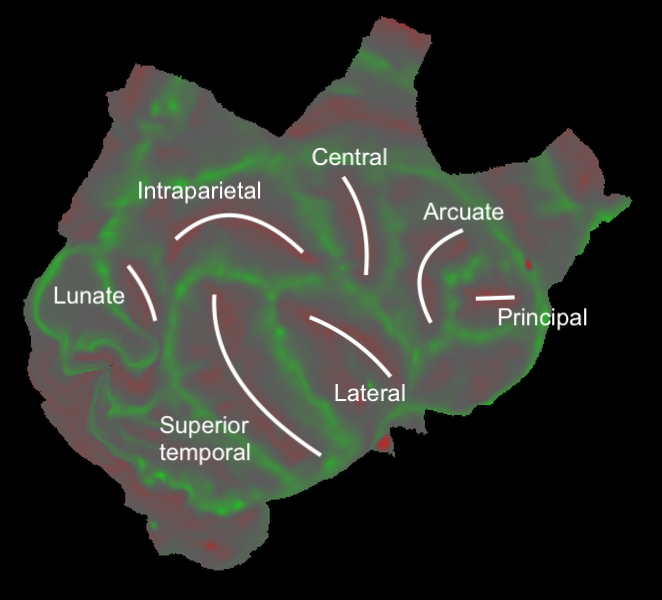
\includegraphics{pics/RH_Flat_Sulci.png}
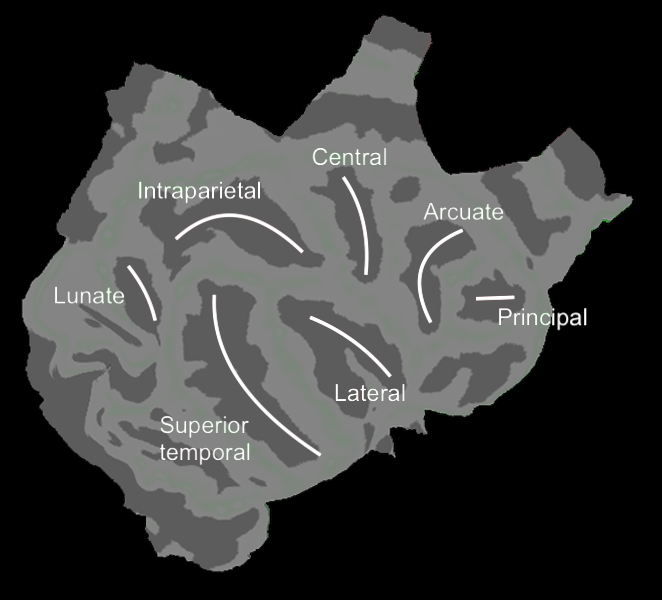
\includegraphics{pics/RH_Flat_Sulci_gray.png}

    \begin{Verbatim}[commandchars=\\\{\}]
{\color{incolor}In [{\color{incolor} }]:} \PY{c+c1}{\PYZsh{} check your result}
        tksurfer \PY{l+s+si}{\PYZdl{}\PYZob{}}\PY{n+nv}{SUBJ}\PY{l+s+si}{\PYZcb{}} rh inflated \PYZhy{}patch rh.full.patch.flat \PYZhy{}curv \PY{c+c1}{\PYZsh{} for a red/green curvature map}
        \PY{c+c1}{\PYZsh{}tksurfer \PYZdl{}\PYZob{}SUBJ\PYZcb{} rh inflated \PYZhy{}patch rh.full.patch.flat \PYZhy{}gray \PYZsh{} for a gray curvature map}
\end{Verbatim}


    \hypertarget{copy-freesurfer-results-back-to-nmt-template-folder}{%
\paragraph{Copy Freesurfer results back to NMT template
folder}\label{copy-freesurfer-results-back-to-nmt-template-folder}}

    \begin{Verbatim}[commandchars=\\\{\}]
{\color{incolor}In [{\color{incolor}15}]:} cp \PYZhy{}r \PY{l+s+si}{\PYZdl{}\PYZob{}}\PY{n+nv}{SUBJECTS\PYZus{}DIR}\PY{l+s+si}{\PYZcb{}}/\PY{l+s+si}{\PYZdl{}\PYZob{}}\PY{n+nv}{SUBJ}\PY{l+s+si}{\PYZcb{}}/surf \PY{l+s+si}{\PYZdl{}\PYZob{}}\PY{n+nv}{fsSurf}\PY{l+s+si}{\PYZcb{}}/surf
\end{Verbatim}


    \begin{Verbatim}[commandchars=\\\{\}]
{\color{incolor}In [{\color{incolor} }]:} \PY{c+c1}{\PYZsh{} return to startpath}
        \PY{n+nb}{cd} \PY{l+s+si}{\PYZdl{}\PYZob{}}\PY{n+nv}{startpath}\PY{l+s+si}{\PYZcb{}}
\end{Verbatim}


    \hypertarget{step-4-create-additional-surfaces-using-connectome-workbench.}{%
\subsection{Step 4: Create additional surfaces using Connectome
Workbench.}\label{step-4-create-additional-surfaces-using-connectome-workbench.}}

This may not be necessary at all. Try the Freesurfer approach and the
conversion to gifti with \texttt{mris\_convert} first (as explained
above)

\hypertarget{requirements}{%
\subsubsection{Requirements}\label{requirements}}

\begin{itemize}
\tightlist
\item
  Connectome Workbench
  (https://www.humanconnectome.org/software/connectome-workbench)
\end{itemize}

    \begin{Verbatim}[commandchars=\\\{\}]
{\color{incolor}In [{\color{incolor} }]:} \PY{c+c1}{\PYZsh{} THIS SHOULDN\PYZsq{}T BE NECESSARY SINCE WE\PYZsq{}RE GETTINGS THESE OUTPUTS ALSO FROM THE FREESURFER PIPELINE !! \PYZsh{}}
        
        \PY{c+c1}{\PYZsh{} set path to where you want the results}
        \PY{n+nv}{wbSurf\PYZus{}path}\PY{o}{=}\PY{l+s+si}{\PYZdl{}\PYZob{}}\PY{n+nv}{NMT\PYZus{}path}\PY{l+s+si}{\PYZcb{}}/single\PYZus{}subject\PYZus{}scans/\PY{l+s+si}{\PYZdl{}\PYZob{}}\PY{n+nv}{SUBJ}\PY{l+s+si}{\PYZcb{}}/wbSurf
        
        \PY{n+nb}{echo} \PY{l+s+s1}{\PYZsq{}Extracting surfaces from segmentation\PYZsq{}}
        \PY{n+nb}{cd} \PY{l+s+si}{\PYZdl{}\PYZob{}}\PY{n+nv}{wbSurf\PYZus{}path}\PY{l+s+si}{\PYZcb{}}
        
        \PY{c+c1}{\PYZsh{} create surfaces}
        IsoSurface \PYZhy{}input \PY{l+s+si}{\PYZdl{}\PYZob{}}\PY{n+nv}{NMT\PYZus{}ss\PYZus{}path}\PY{l+s+si}{\PYZcb{}}/NMT\PYZus{}\PY{l+s+si}{\PYZdl{}\PYZob{}}\PY{n+nv}{SUBJ}\PY{l+s+si}{\PYZcb{}}\PYZus{}process/\PY{l+s+si}{\PYZdl{}\PYZob{}}\PY{n+nv}{SUBJ}\PY{l+s+si}{\PYZcb{}}\PYZus{}segmentation.nii.gz \PY{l+s+se}{\PYZbs{}}
            \PYZhy{}isorois \PYZhy{}o\PYZus{}gii surf
        
        \PY{c+c1}{\PYZsh{} rename to something recognizable}
        mv surf.k2.gii gm.surf.gii \PY{c+c1}{\PYZsh{} gm surface}
        mv surf.k3.gii wm.surf.gii \PY{c+c1}{\PYZsh{} wm surface}
        
        \PY{c+c1}{\PYZsh{} Smooth the surfaces a bit}
        \PY{n+nb}{echo} \PY{l+s+s1}{\PYZsq{}Smoothing the surfaces a bit\PYZsq{}} 
        wb\PYZus{}command \PYZhy{}surface\PYZhy{}smoothing wm.surf.gii \PY{l+m}{0}.5 \PY{l+m}{1} wm\PYZus{}sm.surf.gii
        wb\PYZus{}command \PYZhy{}surface\PYZhy{}smoothing gm.surf.gii \PY{l+m}{0}.5 \PY{l+m}{1} gm\PYZus{}sm.surf.gii
        
        \PY{c+c1}{\PYZsh{} inflate the surfaces}
        \PY{n+nb}{echo} \PY{l+s+s1}{\PYZsq{}Inflating the surfaces\PYZsq{}}
        wb\PYZus{}command \PYZhy{}surface\PYZhy{}generate\PYZhy{}inflated \PY{l+s+se}{\PYZbs{}}
            wm\PYZus{}sm.surf.gii infl\PYZus{}wm\PYZus{}sm.surf.gii vinfl\PYZus{}wm\PYZus{}sm.surf.gii
        wb\PYZus{}command \PYZhy{}surface\PYZhy{}generate\PYZhy{}inflated \PY{l+s+se}{\PYZbs{}}
            gm\PYZus{}sm.surf.gii infl\PYZus{}gm\PYZus{}sm.surf.gii vinfl\PYZus{}gm\PYZus{}sm.surf.gii
        
        \PY{c+c1}{\PYZsh{} view the result in your favorite viewer}
        \PY{n+nb}{echo} \PY{l+s+s1}{\PYZsq{}Inspect the surfaces in a viewer\PYZsq{}}
        freeview \PYZhy{}f wm\PYZus{}sm.surf.gii infl\PYZus{}wm\PYZus{}sm.surf.gii vinfl\PYZus{}wm\PYZus{}sm.surf.gii \PY{l+s+se}{\PYZbs{}}
            gm\PYZus{}sm.surf.gii infl\PYZus{}gm\PYZus{}sm.surf.gii vinfl\PYZus{}gm\PYZus{}sm.surf.gii
\end{Verbatim}



    % Add a bibliography block to the postdoc
    
    
    
    \end{document}
